	%%%%%%%%%%%%%%%%%%%%%%%%%%%%%%%%%%%%%%%%%
%           Fichier maitre				%
%%%%%%%%%%%%%%%%%%%%%%%%%%%%%%%%%%%%%%%%%

\documentclass[a4paper, 12pt, twoside,openright]{report}

%%%%%%%%%%%%%%%%%%%%%%%%%%%%%%%%%%%%%%%%
%           Liste des packages         %
%%%%%%%%%%%%%%%%%%%%%%%%%%%%%%%%%%%%%%%%
%%%%%%%%%%%%%%%%%%%%%%%%%%%%%%%%%%%%%%%%%%%%%%%%%%%%%%%%%%%%%%%%%%%%%
\usepackage{tikz}
\usepackage{pgfplots}
%% Réglage des fontes et typo    
\usepackage[utf8]{inputenc}		% LaTeX, comprend les accents !
\usepackage[T1]{fontenc}
\usepackage{natbib}		% Doit être chargé avant babel
\setcitestyle{authoryear,open={[},close={]}}\usepackage{chapterbib}
%	\renewcommand{\bibsection}{\chapter*{Références Bibliographies}}		% Met les références biblio dan
%s un \section (au lieu de \section*)
 
\usepackage[english,frenchb]{babel}
\usepackage{lmodern}
\usepackage{ae,aecompl}	
\usepackage{multicol}									% Utilisation des fontes vectorielles modernes
\usepackage[upright]{fourier}
\usepackage{lipsum}
\usepackage{wrapfig}
%%%%%%%%%%%%%%%%%%%%%%%%%%%%%%%%%%%%%%%%%%%%%%%%%%%%%%%%%%%%%%%%%%%%%
% Allure générale du document
\usepackage{enumerate}
\usepackage{enumitem}
%\usepackage[section]{placeins}	% Place un FloatBarrier à chaque nouvelle section
\usepackage{epigraph}
\usepackage[font={small}]{caption}
\usepackage[francais,nohints]{minitoc}		% Mini table des matières, en français
	\setcounter{minitocdepth}{2}	% Mini-toc détaillées (sections/sous-sections)
\usepackage[notbib]{tocbibind}		% Ajoute les Tables	des Matières/Figures/Tableaux à la table des matières
%%%%%%%%%%%%%%%%%%%%%%%%%%%%%%%%%%%%%%%%%%%%%%%%%%%%%%%%%%%%%%%%%%%%%
%% Maths                         
\usepackage{amsmath}			% Permet de taper des formules mathématiques
\usepackage{amssymb}			% Permet d'utiliser des symboles mathématiques
\usepackage{mathrsfs}
\usepackage{amsfonts}			% Permet d'utiliser des polices mathématiques
\usepackage{nicefrac}			% Fractions 'inline'
\usepackage{nccmath}
%%%%%%%%%%%%%%%%%%%%%%%%%%%%%%%%%%%%%%%%%%%%%%%%%%%%%%%%%%%%%%%%%%%%%
%% Tableaux
\usepackage{multirow}
\usepackage{booktabs}
\usepackage{colortbl}
\usepackage{tabularx}
\usepackage{multirow}
\usepackage{threeparttable}
\usepackage{etoolbox}
	\appto\TPTnoteSettings{\footnotesize}
\addto\captionsfrench{\def\tablename{{\textsc{Tableau}}}}	% Renome 'table' en 'tableau'
%%%%%%%%%%%%%%%%%%%%%%%%%%%%%%%%%%%%%%%%%%%%%%%%%%%%%%%%%%%%%%%%%%%%%
%% Eléments graphiques                    
\usepackage{graphicx}			% Permet l'inclusion d'images
\usepackage{subcaption}
\usepackage{pdfpages}
\usepackage{rotating}
\usepackage{pgfplots}
	\usepgfplotslibrary{groupplots}
\usepackage{tikz}
	\usetikzlibrary{backgrounds,automata}
	\pgfplotsset{width=7cm,compat=1.3}
	\tikzset{every picture/.style={execute at begin picture={
   		\shorthandoff{:;!?};}
	}}
	\pgfplotsset{every linear axis/.append style={
		/pgf/number format/.cd,
		use comma,
		1000 sep={\,},
	}}
\usepackage{eso-pic}
\usepackage{import}
%%%%%%%%%%%%%%%%%%%%%%%%%%%%%%%%%%%%%%%%%%%%%%%%%%%%%%%%%%%%%%%%%%%%%
%% Mise en forme du texte        
\usepackage{xspace}
\usepackage[load-configurations = abbreviations]{siunitx}
	\DeclareSIUnit{\MPa}{\mega\pascal}
	\DeclareSIUnit{\micron}{\micro\meter}
	\DeclareSIUnit{\tr}{tr}
	\DeclareSIPostPower\totheM{m}
	\sisetup{
	locale = FR,
	  inter-unit-separator=$\cdot$,
	  range-phrase=~\`{a}~,     	% Utilise le tiret court pour dire "de... à"
	  range-units=single,  		% Cache l'unité sur la première borne
	  }
\usepackage[version=3]{mhchem}	% Equations chimiques
\usepackage{textcomp}
\usepackage{array}
\usepackage{hyphenat}
%%%%%%%%%%%%%%%%%%%%%%%%%%%%%%%%%%%%%%%%%%%%%%%%%%%%%%%%%%%%%%%%%%%%%
%% Navigation dans le document
\usepackage[pdftex,pdfborder={0 0 0},
			colorlinks=true,
			linkcolor=blue,
			citecolor=red,
			pagebackref=true,
			]{hyperref}	% Créera automatiquement les liens internes au PDF
					% Doit être chargé en dernier (Sauf exceptions ci-dessous)
%%%%%%%%%%%%%%%%%%%%%%%%%%%%%%%%%%%%%%%%%%%%%%%%%%%%%%%%%%%%%%%%%%%%%
%% Packages qui doivent être chargés APRES hyperref	             
\usepackage[top=2.5cm, bottom=2cm, left=3cm, right=2.5cm,
			headheight=15pt]{geometry}
\usepackage{fancyhdr}
\addtolength{\headheight}{2.5pt}
\fancyhf{}
%\fancyhead[LE,RO]{\nouppercase{\thepage}}
%\fancyhead[L]{\nouppercase{\leftmark}}
\renewcommand{\headrulewidth}{2pt}
\renewcommand{\footrulewidth}{1pt}
\pagestyle{fancy}
\lhead{\nouppercase{\leftmark}}
\rfoot{page \centering \thepage}
\pagestyle{fancy}
\usepackage{tcolorbox}
\usepackage[acronym,xindy,toc,numberedsection,ucmark]{glossaries}
	\newglossary[nlg]{notation}{not}{ntn}{Notation} % Création d'un type de glossaire 'notation'
	\makeglossaries
	\loadglsentries{Glossaire}			% Utilisation d'un fichier externe pour la définition des entrées 
\usepackage{float}% http://ctan.org/pkg/float
\usepackage[linesnumbered,ruled,vlined]{algorithm2e}
\usepackage{algpseudocode}

\usepackage{etex}   

\pgfplotsset{every axis/.append style={
		axis x line=middle,    % put the x axis in the middle
		axis y line=middle,    % put the y axis in the middle
		axis line style={<->}, % arrows on the axis
		xlabel={$x$},          % default put x on x-axis
		ylabel={$y$},          % default put y on y-axis
	},
	cmhplot/.style={color=blue,mark=none,line width=1pt,<->},
	soldot/.style={color=red,only marks,mark=*},
	holdot/.style={color=green,fill=white,only marks,mark=*},
}

\tikzset{>=stealth}


		% Liste des packages et de leurs options
%%%%%%%%%%%%%%%%%%%%%%%%%%%%%%%%%%%%%%%%
%           Commandes perso            %
%%%%%%%%%%%%%%%%%%%%%%%%%%%%%%%%%%%%%%%%
\newcommand{\alp}{\texorpdfstring{\ensuremath{\upalpha}\xspace}{alpha }}
\newcommand{\bet}{\texorpdfstring{\ensuremath{\upbeta}\xspace}{b\'{e}ta }}
\newcommand{\alpbet}{\texorpdfstring{\ensuremath{\upalpha-\upbeta}\xspace}{alpha-b\'{e}ta}}
\newcommand{\alpt}{\ensuremath{\alpha_2}\xspace}
\newcommand{\strt}{\gls{strt}\xspace}
% Tenseur des déformation cylindrique
\newcommand{\epsrr}{\ensuremath{\varepsilon_{rr}}\xspace}
\newcommand{\epstt}{\ensuremath{\varepsilon_{\theta\theta}}\xspace}
\newcommand{\epszz}{\ensuremath{\varepsilon_{zz}}\xspace}
\newcommand{\epsrt}{\ensuremath{\varepsilon_{r\theta}}\xspace}
\newcommand{\epstz}{\ensuremath{\varepsilon_{\theta z}}\xspace}
\newcommand{\epszr}{\ensuremath{\varepsilon_{zr}}\xspace}
\newcommand{\matlab}{\textsc{Matlab}\texttrademark\xspace}
%% Figures centrées, et en position 'here, top, bottom or page'
\newenvironment{figureth}{%
		\begin{figure}[htbp]
			\centering
	}{
		\end{figure}
		}		
%% Tableaux centrés, et en position 'here, top, bottom or page'
\newenvironment{tableth}{%
		\begin{table}[h]
			\centering
			%\rowcolors{1}{coleurtableau}{coleurtableau}
	}{
		\end{table}
		}
%% Sous-figures centrées, en position 'top'		
\newenvironment{subfigureth}[1]{%
	\begin{subfigure}[t]{#1}
	\centering
}{
	\end{subfigure}
}
\newcommand{\citationChap}[2]{%
	\epigraph{\og \textit{#1} \fg{}}{#2}
}
%% On commence par une page impaire quand on change le style de numérotation de pages 
%\let\oldpagenumbering\pagenumbering
%\renewcommand{\pagenumbering}[1]{%
%	\cleardoublepage
%	\oldpagenumbering{#1}
%}
\newcommand{\mcd}{model checking distribué}
\newcommand{\mc}{model checking}
\newcommand{\border}{\emph{Border}}
\newcommand{\ssti}{Search\_ States\_ To\_ Impor}
\newcommand{\notifier}{\emph{Notifier}}
\newcommand{\bn}{\emph{\border{} et \notifier{}}}
\newcommand{\ei}{Etat Interne}
\newcommand{\CDS}{CDS}
\newcommand{\saidouni}{Pr. Djamel Eddine SAIDOUNI}
\newcommand{\bouneb}{Dr. Bouneb Zine El Abidine}
\newcommand{\CDSDef}{Comportemental Distribution States}
\newcommand{\ee}{Etat Externe}
\newcommand{\deplacer}{déplacer}
\newcommand{\dupliquer}{dupliquer}
\newcommand{\parametreone}{\alpha}

\newcommand{\parametretwo}{\beta}
\newcommand{\parametretree}{\gamma}
\newcommand{\parametrefive}{\delta}
\newcommand{\parametrefour}{\gamma m}
\newcommand{\ministere}{R\'{e}publique  Alg\'{e}rienne D\'{e}mocratique et Populaire\\Minist\'{e}re de  l'enseignement Sup\'{e}rieur et de la Recherche Scientifique\\Université Constantine 2 – Abdelhamid Mehri \\Faculté des Nouvelles Technologies de l'Information et la Communication Département d’Informatique Fondamentale et ses Applications}
\newcommand{\sneuf}{\og S9 \fg{}}
\newcommand{\s}[1]{\og #1 \fg{}}
\newcommand{\mone}{\og machine 1 \fg{}}
\newcommand{\mi}{\og machine i \fg{}}
\newcommand{\mj}{\og machine j \fg{}}
\newcommand{\mtwo}{\og machine 2 \fg{}}
\newcommand{\mtree}{\og machine 3 \fg{}}
\newcommand{\curenti}{curent_{iteration}}
\usepackage{amsmath,amsthm}
\usepackage{thmtools}
\theoremstyle{remark}
\newtheorem{Exemple}{Exemple}[section]
\newtheorem{theorem}{Theorem}
\theoremstyle{definition}
\newtheorem{definition}[theorem]{Définition}
\newtheorem{etape}[theorem]{Étape}
\newcommand{\mysection}[2][]
   {\section[#1]
     {\centering #2}
       \setcounter{figure}{0}
       \renewcommand{\thefigure}{\thesection.\arabic{figure}} %Arabic figures
       \renewcommand{\thesection}{\Roman{section}}               %Roman numeral title
}
\newcommand{\mysectionNoNumerotation}[2][]
   {\section[#1]
     {#2}
       \renewcommand{\thesection}{{section}}               %Roman numeral title
}
\setcounter{secnumdepth}{3} 
%Subsections do not get centered
\allowdisplaybreaks
\newcommand{\mysubsection}[2][]
{\renewcommand*{\thesubsubsection}{\thesubsection.\alph{subsubsection}}
\subsubsection[#1]{#2} 
}
\newcommand{\sectionbreak}{\clearpage}
\algnewcommand\algorithmicforeach{\textbf{for each}}
\algdef{S}[FOR]{ForEach}[1]{\algorithmicforeach\ #1\ \algorithmicdo}

%\SetNlSty{}{}{}
\let\oldnl\nl% Store \nl in \oldnl
\newcommand\nonl{%
  \renewcommand{\nl}{\let\nl\oldnl}}% Remove line number for one line
\usepackage{float}
\floatstyle{ruled}
\newfloat{function}{thp}{lop}
\floatname{function}{Function}
\newfloat{procedure}{thp}{lop}
\floatname{procedure}{Procedure}
\newcommand{\frenchAbstract}[1]{\gdef\@frenchAbstract{#1}} 
\newcommand{\frenchAbstractKeywords}[1]{\gdef\@frenchAbstractKeywords{#1}} 
\newcommand{\englishAbstract}[1]{\gdef\@englishAbstract{#1}} 
\newcommand{\englishAbstractKeywords}[1]{\gdef\@englishAbstractKeywords{#1}} 
 %================= configuring minitoc ==================%
%% disabling chapter numbers
\newcommand{\filterminitoc}[1]{#1}
\renewcommand{\thesection}{\csname filterminitoc \endcsname{\arabic{chapter}.}\arabic{section}}
\newcommand{\minitocsection}{\begingroup\renewcommand{\filterminitoc}[1]{}\minitoc\endgroup}
%=============== Customizing Chapters Names ===============%
%@author: Stoufa
%Package pstcol Warning:
%************************************
%(pstcol) The package `pstcol' is obsolet!
%(pstcol) You should use `pstricks' directly:
%(pstcol) \usepackage{pstricks}
%(pstcol) ************************************
%\usepackage{pstcol}
\usepackage{pstricks}
\makeatletter
\def\thickhrulefill{\leavevmode \leaders \hrule height 1.2ex \hfill \kern \z@}
\def\@makechapterhead#1{
	\vspace*{30\p@}%
	{\parindent \z@ \centering \reset@font
		\thickhrulefill\quad 
		\scshape\bfseries\textit{\@chapapp{}  \thechapter}  
		\quad \thickhrulefill
		\par\nobreak
		\vspace*{10\p@}%
		\interlinepenalty\@M
		\hrule
		\vspace*{10\p@}%
		\Huge \bfseries #1 \par\nobreak
		\par
		\vspace*{10\p@}%
		\hrule
		\vskip 50\p@
	}
	\minitocsection
	\thispagestyle{empty}%
	\newpage
}
\def\@makeschapterhead#1{\hbox{%
		\huge\hbox{\textbf{#1}}%
	}\par\vskip 1cm}
\newenvironment{changemargin}[2]{%
	\begin{list}{}{%
			\setlength{\leftmargin}{#1}%
			\setlength{\rightmargin}{#2}%
		}%
		\item[]}
	{\end{list}}

 
 
	% Commandes et environnements perso

%%%%%%%%%%%%%%%%%%%%%%%%%%%%%%%%%%%%%%%%%%
%           Page de Garde		         %
%%%%%%%%%%%%%%%%%%%%%%%%%%%%%%%%%%%%%%%%%%
\makeatletter 
\def\@specialite{Spécialité}
\newcommand{\specialite}[1]{
  \def\@specialite{#1}
}
\def\@directeur{directeur}
\newcommand{\directeur}[1]{
  \def\@directeur{#1}
}
\def\@encadrant{encadrant}
\newcommand{\encadrant}[1]{
  \def\@encadrant{#1}
}
\def\@jurya{}{}{}
\newcommand{\jurya}[3]{
  \def\@jurya{#1,	& #2	& #3\\}
}
\def\@juryb{}{}{}
\newcommand{\juryb}[3]{
  \def\@juryb{#1,	& #2	& #3\\}
}
\def\@juryc{}{}{}
\newcommand{\juryc}[3]{
  \def\@juryc{#1,	& #2	& #3\\}
}
\def\@juryd{}{}{}
\newcommand{\juryd}[3]{
  \def\@juryd{#1,	& #2	& #3\\}
}
\def\@jurye{}{}{}
\newcommand{\jurye}[3]{
  \def\@jurye{#1,	& #2	& #3\\}
}
\def\@juryf{}{}{}
\newcommand{\juryf}[3]{
  \def\@juryf{#1,	& #2	& #3\\}
}
\def\@juryg{}{}{}
\newcommand{\juryg}[3]{
  \def\@juryg{#1,	& #2	& #3\\}
}
\def\@juryh{}{}{}
\newcommand{\juryh}[3]{
  \def\@juryh{#1,	& #2	& #3\\}
}
\def\@juryi{}{}{}
\newcommand{\juryi}[3]{
  \def\@juryi{#1,	& #2	& #3\\}
}
\makeatother 
\newcommand\EtiquetteThese{%
	\put(-10,10){%
		\parbox[t][\paperheight]{\paperwidth}{%
			\hfill
			\colorbox{black}{		
				\begin{minipage}[b]{3em}
					\centering\Huge\textcolor{white}{M\\A\\S\\T\\E\\R\\}
					\vspace{0.3cm}
				\end{minipage}
			}
		}
	}
}

\makeatletter
\newcommand{\pagedegarde}{
\newgeometry{top=2.5cm, bottom=2cm, left=2cm, right=1cm}
 
\AddToShipoutPicture*{\EtiquetteThese}
  \begin{titlepage}
	\centering	
\begin{minipage}{1\textwidth}
	\begin{center}
		\large\ministere{}
	\end{center}				
\end{minipage}


\includegraphics[width=0.2\linewidth]{img/uc2.png}
    \vspace{1cm}
    	\begin{minipage}{1\textwidth}\raggedright
    		\begin{tabular}{>{\bfseries}llr}
			 \large Ann\'{e}e&:\enspace\textbf{\the\year} \\
			 \large \No d'ordre&: \\
			 \large Série&:\\
			\end{tabular}
		\end{minipage}      
    	{\Large{\textbf{M\'EMOIRE}}}\\
    	\vspace{0.5cm}
    	\textit{pour obtenir le diplôme}\\
    	\vspace{0.5cm}
    	{\Large{\textbf{MASTER en Informatique}}}\\
    	\vspace{0.5cm}
    	 {\textbf{Option :} Réseaux et Systèmes Distribués}\\
    \vspace{0.5cm}
    \begin{tcolorbox}[colback=white,boxrule=0pt,toprule=3pt,bottomrule=3pt,arc=0pt,top=0mm,right=0mm,left=0mm,bottom=0mm,boxsep=0.7mm]{
    		\begin{tcolorbox}[colback=white, boxrule=0pt,toprule=1pt,bottomrule=1pt,arc=0pt,enlarge bottom by=-0.9mm, auto outer arc]
    			\centering
    			{\Large\textbf{\@title}}
    		\end{tcolorbox}
    	}
    \end{tcolorbox}
    \vspace{0.5cm}
    	\textit{présentée et soutenue publiquement par}\\
    \vspace{0.5cm}
    	{\Large {\bfseries \@author}} \\
    \vspace{0.5cm}
    	le \today\\   
    %et soutenu publiquement
    \vspace{1cm}
	\begin{tabular}{>{\bfseries}llr}
		\large Encadré par\\
		\@jurya
		\@juryb
		\\ Jury \\
		\@juryc
		\@juryd
	\end{tabular}
	\vfill 
  \end{titlepage}
\restoregeometry  
\nopagebreak  
}
\makeatother
 
%%%%%%%%%%%%%%%%%%%%%%%%%%%%%%%%%%%%%%%%%%%%%%%%%%%%%%%%%%%%%%%%%
%%   			Liste des fichiers à compiler					%
 %%%%%%%%%%%%%%%%%%%%%%%%%%%%%%%%%%%%%%%%%%%%%%%%%%%%%%%%%%%%%%%%%
%	\includeonly{Chapitre1,Chapitre2,Annexes}

% Infos de la page de garde
\author{Karimou Seyni Ibrahim}
\title{. . . . . . . . . . . . . . . . . . . . . . . . . . . . . . . . . . . . . . . . . . . . . . . . . . . . . . . . . . . . . . . . . . . . . .}
\specialite{Réseaux et Système Distribué}
\directeur{Pr. Djamel Eddine SAIDOUNI}
\encadrant{Dr. Bouneb Zine El Abidine}
\date{\today}
\jurya{Pr. Djamel Eddine SAIDOUNI}{Directeur de mémoire}{}
\juryb{Dr. Bouneb Zine El Abidine}{Co-encadreur}{}
\juryc{Dr. L. MEZAI }{Présidente} {}
\juryd{Dr. Chaouche Ahmed-Chawki}{Examinateur}{}
\jurye{. . . . . . . . . . . . . . . . . . . . . . . . . . . . . . . . . . .}{Examinatrice}{}



% Méta-données du PDF
\hypersetup{
    pdfauthor={\@author},
    pdfsubject={Manuscrit de Master},
    pdftitle={\@title},
    %pdfkeywords={space d'états, distribution, modèle checker}
}

\frenchAbstractKeywords{Merci de ne pas dépasser les cinq mots}


\englishAbstractKeywords{Please don't use more than five keywords}

\renewcommand*\listfigurename{Liste des figures}
\begin{document}
	\let\cleardoublepage\clearpage
% Préambule	
	\pagedegarde	
		\pagenumbering{gobble}
\chapter*{}
\vspace{4mm}

\begin{flushright}
	\large
	\textbf{
		A ma mère \\
		A mon père \\
		A toute ma famille\\ A mes ami(e)s
	} 
\end{flushright}

\vspace{8mm}
\chapter*{Remerciements}
Je tiens tout d’abord à remercier Allah, le Clément, le miséricordieux qui nous a permis de mener à bien ce modeste travail.
\\\\
En premier lieu, je tiens à exprimer ma sincère gratitude à mon encadreur\\ \textbf{\saidouni{}}, pour son intégrité, sa disponibilité, sa générosité de partager ses connaissances. Je voudrais lui témoigner ici toute ma gratitude pour m'avoir guidé durant ces périodes et laisse entrevoir ce que le mot recherche veut dire.
\\\\
Je remercie chaleureusement \textbf{\bouneb{}} pour avoir accepté d'être mon co-encadreur, pour son soutien, ses nombreux conseils et l'intérêt qu'il a porté à mon travail.
\\\\
Je souhaite exprimer toutes ma reconnaissance à mes parents qui m'ont soutenu tout au long de ces années et m'ont toujours encouragé de faire ce que je souhaitais et de donner le meilleur de moi-même. 
\\\\
Mes plus vifs remerciements s’adressent à tous les corps enseignants pour leur patience, leur dévouement pour nous avoir apporté le bagage nécessaire.
\\\\
Je voudrais aussi exprimer mon amitié aux personnes avec qui j'ai eu le plaisir de partager ses années d'études et surtout ceux du premier et du second cycle.

	
		\pagenumbering{gobble}
\chapter*{}
\begin{changemargin}{3mm}{0cm}
    \begin{minipage}[c]{0.96\columnwidth}        

        \selectlanguage{french}
        
        {\LARGE\textbf{Résumé}}
        \vskip1mm
            \begingroup
                La vérification formelle constitue une étape indispensable pour garantir le bon fonctionnement des systèmes complexes et critiques. Le model checking est une technique efficace pour vérifier des propriétés sur des systèmes décrit avec un modèle formel. Ce pendant, cette méthode de vérification souffre d'un problème majeur engendré par l'explosion combinatoire de l'espace d'états à explorer  dans un temps raisonnable.
                \\\\
                Pour merdier a ce problème, la distribution de l'espace d'états est la solution la plus rependus  en vue de tirer profit de la quantité de mémoire et de la puissance de calcul disponibles sur chaque machine. Par contre aboutir à une meilleur distribution pour accélérer la vérification s'avère être difficile a réalisé.\\
                
                Notre travail réside dans la distribution de l'espace d'états, pour établir un compromis entre l’équilibrage de charge des différentes machines et la minimisation du taux de communications. Pour cela, nous proposons une nouvelle approche de distribution en avale de l'espace d'états basée la théorie de jeux et l'analyse des états. L’approche proposée vise à analyser l'espace d’états tout en extrayant les informations pertinentes sur les états. Ensuite, redistribuer les états suite à leurs pertinences soit migrés définitivement soit dupliqués sur d’autres machines, afin de minimiser le nombre de communications entre les machines. Cela est fait grâce à une stratégie comportementale de la théorie de jeux au quelle les machines cherchent à optimiser leur taux de communications tout en maintenant l'équilibrage de charge entre les machines à l’aide de seuils prédéfinis pour chaque machine. Ceci permet à une application d'optimiser ses comportements en cumulant ses expériences d’exécutions, ainsi grâce à l'utilisation des bases de données orientés graphes, les prochaines exécutions de l’application seront fait à partir des améliorations gagnées précédemment.
            \endgroup
        \vskip1mm
        {\textbf{Mots clés : }
            \begingroup
                Réseau de Petri, Calcul parallèle, Structure de Kripke Distribué, Model checking distribué, Distribution des espaces d'états, 
                Génération de l’espace d’états, Méthodes d’optimisation, Théorie de jeux.
            \endgroup
        }
    \end{minipage}    
\end{changemargin}
\break
        
\pagenumbering{gobble}
\chapter*{}
\begin{changemargin}{3mm}{0cm}
	\begin{minipage}[c]{0.96\columnwidth} 
		\selectlanguage{english}
		{\LARGE\textbf{Abstract}}
		\vskip1mm
		\begingroup
		Formal verification is an essential step for ensuring the proper functioning of complex and critical systems. Model checking is an effective technique for checking properties on systems described with a formal model. However, this verification method suffers from a major problem caused by the combinatorial explosion of the states space to be explored in a reasonable time.
		\\
		
		To solve this problem, the states space distribution is the most common solution to take advantage of the amount of memory and computing power available on each machine. On the other hand, it is difficult to obtain a better distribution to accelerate the calculation of the verification.
		\\\\
		Our work lies in the distribution of states space, to establish a compromise between the load balancing of the different machines and the minimization of the communication rate. For this, we propose a new distribution approach in downstream of the states space based game theory and states analysis. The proposed approach aims to analyze the states space while extracting relevant state information. Then, redistribute the states following their relevance either migrated permanently or duplicated on other machines, in order to minimize the number of communications between the machines. This is done through a behavioral strategy of game theory in which machines seek to optimize their communications rate while maintaining load balancing between machines using predefined thresholds for each machine. This allows an application to optimize its behavior by combining its execution experiences, and thanks to the use of graph-oriented databases, the next executions of the application will be made from the improvements previously gained.		
		\endgroup
		\vskip1mm
		{\textbf{Keywords : }
			\begingroup			
			Petri Net, Parallel Computing, Distributed Kripke Structure, Distributed Model Checking, State Space Distribution,	State Space Generation, Optimization Methods, Game Theory.
			\endgroup
		}
    \end{minipage}    
\end{changemargin}
	\clearpage
	\pagenumbering{roman}
	% Table des matières
		\setcounter{tocdepth}{1}	% Pas besoin de trop détailler le sommaire ici (chapitres/sections)
		\dominitoc						% Génération des mini-toc	\pagenumbering{arabic}
		\tableofcontents
	% Liste des figures
		\listoffigures
		\listoftables
		\clearpage
%%%%%%%%%%%%%%%%%%%%%%%%%%%%%%%%%%%%%		
%        Contenu du document        %
%%%%%%%%%%%%%%%%%%%%%%%%%%%%%%%%%%%%% 
	\setcounter{mtc}{3}	% "Corrige" les minitocs décallés à cause des chapter* (ex : table des matières)	
	\pagenumbering{arabic}
	\addcontentsline{toc}{part}{Introduction Générale}
\markboth{Introduction Générale}{}
\chapter*{Introduction Générale}
\section*{Introduction} 	
Les progrès fulgurants des Technologies de l’Information et de la Communication({\emph{TIC}}) et le bésoin de faire collaborer des objets ont conduit à un concept moderne qui est « Internet of Things» (\emph{IoT}). L'IoT nous offre une nouvelle opportunité de croissance nous permettant délimiter la perte de temps, de ressource, améliorant ainsi nos vie quotidiennes. De nos jours, il existe de nombreuses plateformes et applications pour l’IoT conduisant à fournir de nouveaux services et automatiser de nombreux processus dans l'industrie(smart industry), la santé(smart health), le ménage, les transports(smart transport) et de nombreux autres secteurs.

Il existe plusieurs définitions sur le concept de l’IoT, mais nous adoptons celle proposée par Weill et Souissi qui ont défini l’IoT comme « une extension de l'Internet actuel envers tout objet pouvant communiquer de manière directe ou indirecte avec des équipements électroniques eux-mêmes connectés, à l'Internet. Cette nouvelle dimension de l'Internet s'accompagne avec de forts enjeux technologiques, économiques et sociaux tout en assurant la protection des données des utilisateurs » \citep{refdiot}. Quasiment n'importe quel appareil doté d'un bouton marche/arrêt peut se connecter à l'Internet aujourd'hui, intégrant ainsi la catégorie des objets de l'IoT \citep{ciscorefiot} 

En ce qui concerne l'IoT, Les objets connectés peuvent être des objets  physiques ou virtuelles (smartphones, ordinateurs, data centers, réseaux Wi-Fi, réseaux cellulaires, puces RFID , capteurs, équipement ménager, montres, serrures, véhicules, drones, etc ) pouvant être identifiés et intégrés dans la communication des réseaux.
D'après la plateforme statisca \citep{refstatic} aujourd'hui le nombre d'objets connectés est estimé à $30.73 milliards$ d'objets connectés dans le monde et ce nombre atteindrait les $75.44\; milliards$ d'objets connectés en $2025$.

Cependant assurer la confidentialité, la disponibilité et l'intégrité des objets connectés ainsi que les données qui y transitent sont les principales préoccupations concernant l'adoption de ce nouveau concept l'IoT. Une fois que les appareils sont connectés à Internet, ils deviennent vulnérables à d'éventuelles d'attaques informatiques. l'IoT étant la prochaine génération  d'Internet \citep{cisco} avec de plus en plus d'objets connectés allant des villes connectés aux vaches connectées. Dans ce réseau les objets connectés s’échangent des informations pour répondre à un but bien défini. Cette collaboration des objets ouvre des portes d’attaques aux hackers qui effectuent des attaques de plus en plus sophistiquées.

Selon $451$ Research \citep{ref451rec} beaucoup d'entreprises sont toujours retissant dans l'adoption de l'IoT à cause sa gestion de la sécurité de ce nouveau qui est encore en état embryonnaire, mais $55\%$ des entreprises qui ont adoptées l'IoT classent la gestion de la sécurité IoT comme leur priorité absolue lors des déploiements de projets IoT au sein de leurs organisations. Les systèmes vulnérables des objets connectés  peuvent être compromis de n’importe où et utilisés pour cibler n’importe qui raison pour laquelle la sécurité IoT est une préoccupation mondiale.

{\green Les objets connectés font faces à plus types de menaces. ces types de menaces sont classées en quatre($4$) types \citep{refinfosec} : 
\begin{itemize}
\item \textbf{Déni de Service :} Cette menace vise la disponibilité d'un service ou d'une ressource en la saturant de requête indésirable empêchant ainsi ses utilisateurs légitimes de l'utiliser. cette indisponibilité du service ou d'une ressource est mise en œuvre avec par l'attaque de types DDoS. C'est probablement l'une des ménaces les plus courantes et les plus dangereuses . 
\item \textbf{les logiciels malveillants} Un auteur de malware conçoit spécifiquement ses codes pour compromettre les architectures utilisées par les appareils IoT. Un code malveillant pourrait être utilisé pour infecter les ordinateurs utilisés pour contrôler un réseau d'appareils intelligents ou pour compromettre le logiciel qui y est exécuté. Dans ce deuxième scénario, les attaquants peuvent exploiter la présence d'une faille dans le micrologiciel exécuté sur les appareils et exécuter leur code arbitraire, transformant les composants IoT en utilisation non planifiée \citep{refinfosec}
\item \textbf{Violation de données (Data Breaches) : } C'est une menace visant l'intégrité et la confidentialité des données. les attaquants peuvent utiliser des attaques de type homme du milieu pour intercepter les communications des objets connectés.  
\item \textbf{Affaiblissement des périmètres : } Les appareils de l'Internet des objets ne sont généralement pas conçus pour la sécurité. Bien qu'il s'agisse d'appareils connectés à Internet, la majorité des appareils ne disposent pas de mécanismes de sécurité réseau. Prenons, par exemple, un compteur intelligent. Si l'attaquant est en mesure de le compromettre, il pourrait avoir accès à notre réseau domestique, nous espionner ou causer des dommages physiques à notre environnement domestique. Le problème est tout aussi grave si nous considérons l'utilisation d'appareils IoT dans n'importe quelle industrie.\citep{refinfosec}
\end{itemize}
}
\section*{Contribution}
{\red
Nous nous focaliseront dans ce mémoire sur la menace « déni de service », notamment l'attaque par Déni de Service Distribué (\emph{DDoS}). Une attaque par déni de service distribué est une attaque qui empêche l'accès à une ressource ou à un service internet. Elle est obtenue en saturant avec des centaines de milliers voire des millions de connexions(requêtes) un serveur ou un objet connecté jusqu'à le bloquer.

\textbf{À titre d'exemple : } 
\begin{itemize}
	\item En $2007$ l'Estonie \citep{refestonie} a été victime de la première plus grande attaque DDoS de l'histoire. l'attaque visait le système informatique du pays notamment ses sites gouvernementaux, ses banques et ses médias créant la panique et déclenchant de vaste d'émeute au sein de la population et force de l'ordre. 
	\item En octobre $2016$ \citep{refddos} Dyn un important fournisseur de service de noms de domaine a été victime d'une vague d'attaque par déni de service distribuée. l'attaque était orchestrée à l'aide d'un logiciel malveillant appelé Mirai, les pirates se sont servis de ce programme pour créer un énorme botnet de $100000$ objets connectés pour lanceur leur attaque. L'attaque a été extrêmement perturbatrice et a fait tomber les sites Web de plus de $80$ de ses clients, notamment Amazon, Netflix, Airbnb, Spotify, Twitter, PayPal et Reddit. Les dommages causés par cette attaque auraient coûté $110 millions$ de dollars ainsi que la dégradation de la réputation du fournisseur.
	\item En 2018 github, une plateforme de développement à son tour était visée d'attaque DDoS qui a été. l'attaque a été maitrisée 10 min après \citep{refddos} grâce à la présence système de protection d'attaque DDoS dans la plateforme.  
\end{itemize}
}

Nous proposons dans ce mémoire la mise en place d'un système de détection d'intrusion dans le réseau IoT contre les attaques de types DDoS. Afin d'assurer la disponibilité d'un service ou d'un objet connecté dans le réseau IoT. Notre choix du DDoS s'explique du fait que le DDoS utilise les objets connectées non sécurisés pour sa mise œuvre et du fait qu'elle est actuellement considérée comme l'attaque la plus dangereuse visant l'IoT \citep{8355541} \cite{inproceedings}.

\section*{Plan du document}
Conformément à ce qui vient d’être exposé, le manuscrit se décompose en deux parties :
\begin{description}
\item[La première partie :] présente l'état de l'art sur les différents domaines entrant en jeu dans le cadre de ce mémoire à savoir la sécurité informatique et la cybersécurité, l'attaque par déni de service distribué (\textbf{DDoS}), l'Internet des objets(\textbf{l'IoT}).
\item[La seconde partie :] 
\end{description}
	\clearpage
 	\part{Contexte de travail}
	\clearpage
	\nopagebreak
	    
\chapter{Sécurité informatique et Cybersécurité} 
\section{Introduction}
\parindent=0.2cm 
Dans un monde de plus en plus connecté, où l’économie mondiale dépend de plus en plus de l’utilisation des services d’Internet, des services numériques, ainsi que les technologies émergentes sont davantage ancrées dans les économies du monde, il est absolument essentiel d'assurer une cybersécurité efficace. Tant que l'utilisation des TIC progressent, les risques augmentent aussi. Il s'agit donc de répondre à des défis et des cybermenaces qui ne cessent d'évoluer, ce qui exige que tous les acteurs soient au courant des facteurs de risque, qu'ils disposent des capacités nécessaires et qu'ils prennent les mesures appropriées en matière de prévention et de résolution. Pour garantir un cyberespace sûr, résilient et sécurisé les pays doivent explorer la réalité complexe et multisectorielle de la cybersécurité ce qui soulève des questions stratégiques, techniques, juridiques, de politique et de sécurité, et qui suppose l'établissement d'une collaboration multisectorielle et internationale.\\

Aujourd’hui notre mode de vie ultra connecté ne peut se passer des objets connectes et comme une connexion à un réseau rend possible une intrusion. Le fait d’interconnecter des objets augmentent d’autant plus la surface d’attaque aux cyber attaquants nous rendant ainsi beaucoup plus vulnérables.Cette multiplicité d’objets, de connexions, et de règlementation fait qu’aujourd’hui qu’il est difficile d’appliquer un seul modèle de sécurité. Le cyber espace est donc un monde à hauts risques d’attaques. Le mot anglais « Security » signifie une résistance à une malveillance, se traduit en français par « sûreté », alors que le mot « safety » signifie une résistance à une panne.\\

\textbf{La sécurité informatique} est l’ensemble des moyens techniques, organisationnels, juridiques et humains nécessaires mis en oeuvre pour réduire la vulnérabilité d’un système contre les menaces accidentelles ou intentionnelles. C’est une branche de la technologie de l’information qui étudie et met en oeuvre les menaces et les vulnérabilités des systèmes informatiques.\\
\textbf{La cybersécurité} est la partie de la sécurité informatique qui assure la protection du cyberespace contre les cybers menaces. Le terme cybersécurité n’est pas synonyme de sécurité informatique (1). La cybersécurité s’applique aux systèmes interconnectés, du fait que l’information numérique à protéger voyage à travers eux et y réside en eux. (2).\\

\section{Les objectifs de sécurité informatique }
La notion de sécurité d’un système informatique s’exprime généralement en termes de \textbf{disponibilité (D), d’intégrité (I) et de confidentialité (C) (3)}. Ces critères (dits critères DIC) sont les objectifs de sécurité de base dont leurs mises en oeuvre permettent d’atteindre un certain niveau de sécurité. En plus de ces fonctions s’ajoutent d’autres services de sécurité complémentaires pour confirmer \textbf{la véracité ou l’authenticité}  d’une action ou d’une ressource (notion d’authentification) ou encore pour prouver l’existence d’une action à des fins de \textbf{non-répudiation ou d’imputabilité}, ou de \textbf{traçabilité}.\\

Un service de sécurité est un service qui augmente la sécurité des traitements et des échanges de données d’un système. Les critères de disponibilité, de confidentialité et d’intégrité sont à satisfaire par des mesures appropriées afin de pouvoir atteindre un certain niveau de confiance dans les contenus et le fonctionnement des infrastructures informatiques et télécoms.
%\cia

\subsection{La confidentialité : }
La confidentialité consiste à rendre l'information inintelligibles aux acteurs illégitimes d’une transaction ou d’une communication. Elle garantit l’anonymat des données en limitant leurs accès par le chiffrement et l’authentification.\\
La confidentialité assure que seules les personnes autorisées peuvent accéder à l’information. Les politiques d’entreprise devront limiter l’accès à l’information au personnel autorisé et garantir que seules ces personnes autorisées consultent ces données. Les données peuvent être compartimentées selon le niveau de sécurité ou de
sensibilité de l’information.\\
Par ailleurs, les employés doivent suivre une formation pour comprendre les bonnes pratiques en matière de protection des informations sensibles pour se protéger et pour protéger l’entreprise contre les attaques. Il existe deux méthodes complémentaires permettant d’assurer la confidentialité :
\begin{itemize}[label=\textbullet]
	\item Limiter et contrôler l’accès aux données afin que seules les personnes habilitées à les lire ou à les modifier puissent le faire.
	\item Rendre inintelligibles les données en les chiffrant de telle sorte que les personnes qui ne sont pas autorisées à les déchiffrer ne puissent les utiliser. Cette tache est réalisée en utilisant le chiffrement (cryptographie).
\end{itemize}
\subsection{L’intégrité :}
Vérifier l’intégrité des données consiste à déterminer si les données n'ont pas été altérées durant la communication. L’intégrité représente l’exactitude, la cohérence et la fiabilité des données pendant tout leur cycle de vie. Le critère d’intégrité des ressources physiques et logiques (équipements, données, traitements, transactions, services) assure qu’elles demeurent intactes, qu’elles n’ont pas été détruites ou modifiées à l’insu de leurs propriétaires tant de manière intentionnelle, qu’accidentelle.\\

Préserver l’intégrité des ressources et s’assurer que des ressources sont intègres sont l’objet de mesures de sécurité. Ainsi, se prémunir contre l’altération des données et avoir la certitude qu’elles n’ont pas été modifiées collabore à la qualité des prises de décision basées sur celles-ci. Si en télécommunication, l’intégrité des données relève essentiellement de problématiques (4)liées au transfert de données, elle dépend également des aspects purement informatiques de traitement de l’information (logiciels d’application, systèmes d’exploitation, environnements d’exécution, procédures de sauvegarde, de reprise et de restauration des données). L’intégrité des données est mise en oeuvre par des mécanismes cryptographiques et les signatures numériques pour s’assurer que les données n’ont pas été victimes d’écoute ou d’altération lors de leur transfert par des cyberattaques
\subsection{La Disponibilité :}
La disponibilité d’une ressource est relative à la période de temps pendant laquelle le service qu’elle offre est opérationnel. Elle garantit la continuité à l’accès à un service ou à des ressources. Le volume potentiel de travail susceptible d’être pris en charge durant la période de disponibilité d’un service détermine la capacité d’une ressource à être utilisée. Il ne suffit pas qu’une ressource soit disponible, elle doit pouvoir être utilisable avec des temps de réponse acceptables. Sa disponibilité est indissociable de sa capacité à être accessible par l’ensemble des ayants droit (notion d’accessibilité).\\

La disponibilité des services, systèmes et données est obtenue par une maintenance des équipements, la réparation des matériels, la mise à jour des systèmes d’exploitation et des logiciels, la création de sauvegardes ainsi que l’utilisation d’équipements ou de service de sécurité. Les attaques de types \textbf{DoS} et \textbf{DDOS}  peuvent causer l’indisponibilité d’un service ou d’une ressource. Celles-ci, sont possibles si les procédures de sauvegarde et de restitution ainsi que les supports de mémorisation associés ne sont pas gérées correctement ou s’il y a malveillance. Une politique de sauvegarde et des systèmes de détection d’attaques de types \textbf{DDOS} doivent être mis en oeuvre pour éviter le risque d’indisponibilité d’un service ou d’une ressource.
\subsection{La traçabilité : }
L’enregistrement des activités permettent la traçabilité des événements et leur analyse. Garder la mémoire des actions survenues permet notamment de reconstituer et de comprendre ce qui s’est passé lors d’incidents afin d’améliorer la sécurité, d’éviter que des erreurs ne se répètent ou d’identifier des fautifs. Cela autorise par exemple d’analyser le comportement du système et des utilisateurs à des fins d’optimisation, de gestion des incidents et des performances ou encore d’audit.\\
L’enregistrement des actions et événements permet également d’enrichir les bases de données qui permettent de développer des applications de surveillance, de détection et de réaction aux incidents, en particulier à l’aide des techniques issues de l’intelligence artificielle.
\subsection{L’authentification et l’identification :}
L'identification consiste à attribuer une identité unique à un utilisateur. Elle permet de répondre à la question : \textit{Qui êtes-vous ?}\cite{ref5}. Pour se faire l'utilisateur utilise un identifiant unique qu’on nomme Compte d'accès (Nom d'utilisateur ou Login en anglais). L’authentification consiste à assurer la véracité de l'identité d'un utilisateur. Elle permet de répondre à la question : \textit{êtes-vous réellement cette personne ?} \cite{ref5} Pour se faire l’utilisateur utilise un authentifiant ou code secret (mot de passe ou password en anglais) dont lui seul à la connaissance.\\
L’identification et l’authentification des ressources et des utilisateurs permettent d’associer la réalisation d’une action à une entité qui pourra en être tenue responsable et éventuellement en rendre compte. Un contrôle d'accès permet l'accès à des ressources uniquement aux personnes autorisées à travers un mot de passe crypté.
%\authenti
\subsection{La non-répudiation et l’imputabilité : }
\textbf{La non-répudiation} de l'information est la garantie qu'aucun des correspondants ne pourra nier une transaction, c'est-à-dire de garantir à chacun des correspondants que son partenaire est bien celui qu’il prête être en d’autres termes assurer la preuve d’origine ou de destination de message.\\
\textbf{L’imputabilité} est la possibilité d’attribuer la responsabilité d’une infraction à un individu. Elle peut être réalisée par un ensemble de mesures garantissant l’enregistrement fiable d’informations pertinentes relatives à un événement. La non-répudiation et l’imputabilité sont assurer en utilisant les algorithmes de chiffrement asymétriques.
\section{Application de la sécurité informatique : }
La sécurité contient une variété de contextes et dépends du domaine d’application. On distingue 6 catégories de sécurité en fonction du domaine d’application (Figure 3) :
\begin{itemize}[label=\textbullet]
\item \textbf{Sécurité matérielle physique et environnementale};
\item \textbf{Sécurité logique et applicative};
\item \textbf{Sécurité de l’information} ;
\item \textbf{Sécurité de l’exploitation} ;
\item \textbf{Sécurité des réseaux };
\item \textbf{Cybersécurité}.
\end{itemize}
%\imageAPS
\newpage
\subsection{La cybersécurité :}
Le mot \emph{Cybernétique} vient du grec « kuberneïn » qui signifie \textit{diriger ou gouverner}, terme repris en 1948 par le mathématicien \textbf{Norbert Wiener} ancien professeur du Massachusetts Institute de Technologie (MIT) qui l’a publié pour la première fois dans son ouvrage intitulé Cybernetics, or Control and Communication in the Animal and the Machine\cite{cybernetics}.\\
Plusieurs décennies plus tard l’auteur de science-fiction William Gibson utilise le terme de cyberespace dans son roman le Neuromanien. Il s’agit d’une trilogie qui a pour personnage central un voleur de données. Celui-ci est à mesure d’établir des connexions entre son esprit et un réseau mondial liant des ordinateurs entre eux \cite{neuromacer}.\\
Au fuir du temps le préfixe \textit{cyber} va participer ainsi à la construction de nouveaux mots lui donnant une nouvelle définition. Cyber est un préfixe servant de créer de mots relatifs à l’utilisation d’internet et à cette société de l’information qui a vu le jour à la fin du XXème. Aujourd’hui il y a plus de 40 mots débutants par Cyber dont : Cybersécurité, cybernétique, cyberespace, cybercafé, cybercrime, cyberattaque, cyberdéfense, cyberguerre, cyberterroriste, cybermonde etc.\\
Aujourd’hui avec l’utilisation extensif d’Internet des objets générant de nouveaux types de menaces dont seule la cybersécurité peut y faire face.\\

La cybersécurité est la partie de la sécurité informatique qui protège le cyberespace contre les cybers attaques. Elle concerne la sécurité des systèmes accessibles via le cyberespace(internet)et englobe la sécurité de l’information, la sécurité des réseaux et des environnements connectés. Le cyberespace est un espace virtuel relatif à notre espace naturel en d’autres termes un ensemble d’infrastructures numériques, de données et services misent en réseaux mais contrairement à la terre, à la mer, à l’air et à l’espace-extra atmosphérique, le cyberespace est une pure création de l’être humain qui ne relève pas de la nature \cite{ref4}. Le terme cybersécurité est large et englobe chaque élément, de la sécurité de l’ordinateur à la reprise de l’activité après sinistre et la formation des utilisateurs \cite{ref8}
\subsection{La sécurité des réseau : }
La sécurité d’un réseau consiste à protéger un réseau informatique contre les intrus, qu'il s'agisse d'attaques ciblés ou de logiciels malveillants en d’autres termes protéger les équipements, les applications et les données du réseau contre les cybers attaques. Elle utilise plusieurs services et protocoles de défense allant de la couche physique à la couche application. Pour se faire plusieurs approches sont utilisés dans le modèle \textbf{TCP/IP} comme décrit ci-dessous :
\begin{itemize}[label=\textbullet]
\item Couche transport (protocoles TLS/SSL, SSH),
\item Couche internet (protocole IP Sec);
\end{itemize}
\subsubsection{Protocoles TLS/SSL :}
\textbf{TLS} de l’acronyme \textbf{T}ransport \textbf{T
L}ayer \textbf{S}ecurity et \textbf{SSL} de l’acronyme \textbf{S}ecure \textbf{S}ocket \textbf{L}ayer, sont des protocoles de chiffrement qui garantissent la sécurité des échanges de données via un réseau informatique. Ils sont largement utilisés pour la sécurisation des communications sur internet.\\
Ils utilisent les techniques de chiffrements asymétriques et des algorithmes de cryptage comme RSA, ECC, pour assurer la confidentialité, l’intégrité des données ainsi que l’authentification et l’identification des utilisateurs.
\subsubsection{Le protocole IPSec :}
IP Sec pour Internet Protocol Security est une suite de protocoles normalisés par L’Internet Engineering Task Force (\textbf{IETF}) qui fournit des services de sécurisations des données dans un réseau IP au niveau de la couche réseau. Fondé dans le but d’assurer la sécurité du protocole IPv6 et a été réadapter par la suite au protocole IPv4. Il assure les critères de confidentialité, d’authentification et d’intégrité des données échangées à travers un réseau IP ainsi qu’à la création de réseau privé virtuel (\textbf{VPN}).\\
L’\textbf{IPSec} peut fonctionner en deux : mode transport et mode tunnel. Le mode transport est utilisé pour les communications de bout en bout (Host to Host). Le mode tunnel est utilisé pour les configurations passerelle à passerelle ou passerelle à hôte (Gate-to-Gate ou host-to-Gate)\cite{ref9}.\\

En plus de ces protocoles il existe plusieurs moyens classiques pour protéger un réseau informatique dont : les firewalls, la segmentation du réseau, les anti-virus et anti-malwares, les contrôles d’accès réseaux, les zones démilitarisés (DMZ) dont nous détaillerons dans la section mécanismes de sécurité.
\subsection{La sécurité logique et applicative :}
La sécurité des applications se concentre sur la protection des logiciels et des appareils contre les menaces. Une application compromise pourrait fournir un accès aux données qu'elle est destinée à protéger. Une sécurité réussie commence au stade de la conception, bien avant le déploiement d'un programme ou d'un périphérique.\\
La sécurité logique fait référence à la réalisation de mécanismes de sécurité par logiciel contribuant au bon fonctionnement des programmes, des services offerts et à la protection des données. Elle s’appuie généralement sur :
\begin{itemize}
\item La qualité des développements et l’implémentation des logiciels et des tests de sécurité ;
\item Une mise en oeuvre adéquate de la cryptographie pour assurer intégrité et confidentialité ;
\item Des procédures de contrôle d’accès logique, d’authentification ;
\item Des procédures de détection de logiciels malveillants, de détection d’intrusions et d’incidents ;
\item La sécurité applicative comprend le développement pertinent de solutions logicielles (ingénierie du logiciel, qualité du logiciel) ainsi que leur intégration et exécution harmonieuses dans des environnements opérationnels.
\end{itemize}
\subsection{La sécurité des informations : }
La sécurité de l'information est un ensemble de stratégies de gestion et politiques de sécurités visant à protéger, détecter, recenser et contrer les menaces ciblant les données. Une donnée est la représentation d’une information. Elle vise à protéger des données et s'applique à tous les aspects de la sûreté, l'intégrité, la disponibilité et la confidentialité, la garantie, et la protection d'une donnée ou d'une information quelle que soit sa forme, tant en stockage qu'en transit \cite{ref8}.\\

Le système d’information étant le maillon de l’entreprise, l’information qui y transite doit être impérativement protéger contre le vol, la destruction et la falsification d’information pouvant causer d'énorme pertes à l’entreprise. Une classification des données permet de qualifier leur degré de sensibilité (normale, confidentielle, etc.) et de les protéger en fonction de ce dernier
\subsection{La sécurité d'exploitation : }
La sécurité de l'exploitation est un ensemble de stratégies de gestion et de politiques de sécurités visant à assurer le bon fonctionnement opérationnel des systèmes informatiques. Cela comprend la mise en place d'outils et de procédures relatifs aux méthodologies d'exploitation, de maintenance, de test, de diagnostic, de gestion des performances, de gestion des changements et des mises à jour\cite{ref4}. Elle s'appuie sur les différents mécanismes et services de sécurités suivants :
\begin{itemize}[label=\textbullet]
\item Une gestion des systèmes d’exploitation, des configurations et des mises à jour ;
\item Gestion des incidents et suivi jusqu’à leur résolution ;
\item Une politique de sauvegarde, de secours, de continuité et de tests;
\item Gestion des contrats de maintenance ;
\item Une analyse des fichiers de journalisation et de comptabilité 
\end{itemize}
\section{Les types de menaces et d’attaques : }
Une menace est une cause potentielle d’incident, qui peut provoquer un dommage sur un système et ayant un impact sur ses fonctionnalités, son intégrité ou sa disponibilité. Une cybermenace est une menace qui s’exprime via le cyberespace, qui peut toucher tout système connecté à Internet dont sa concrétisation par une cyberattaque, peut affecter le bon fonctionnement des ordinateurs, des réseaux de télécommunication et de tous les services et activités humaines qui en dépendent. Les cybermenaces sont le plus souvent associées à l’usage malveillant des technologies Internet et à la cybercriminalité. De nombreuses cyberattaques existent, elles recouvrent des réalités diverses en fonction des cibles touchées, de leurs impacts, finalités, origines et auteurs.
\subsection{La cybercriminalité : }
Selon Colin ROSE « La cybercriminalité est la troisième grande menace pour les grandes puissances, après les armes chimiques, bactériologiques, et nucléaires » \cite{ref10}. Le cout global de la cybercriminalité est estimé à 6000 milliards de dollars et triplera le nombre d’emplois non pourvu en cybersécurité d’ici 2021 \cite{ref1112}.\\
\textbf{La cybercriminalité} est toute infraction impliquant l’utilisation des technologies informatiques. Elle comprend des acteurs uniques ou des groupes ciblant des systèmes à des fins de gain financier ou de perturbation. Malgré que les entreprises et les forces de l’ordre tentent de s’attaquer au problème croissant, le nombre de cybercriminels continue de croître, profitant de l’anonymat d’Internet.\\
La cybercriminalité se divise en trois grandes catégories : la cybercriminalité individuelle, la cybercriminalité contre la propriété et la cybercriminalité gouvernementale \cite{ref1112}
\begin{description}
\item[La cybercriminalité individuelle] est une catégorie de cybercriminalité dont le criminel utilise des informations et programmes malveillants pour arriver dans le but de nuire à un individu.
\item[La cybercriminalité contre la propriété] est la catégorie de cybercriminalité dont le criminel s’usurpe (vol d’identité) de l’identité d’une personne. Une fois le criminel possède les informations personnelles volées il procède à des achats, des élévations de privilèges afin d’accéder à des informations confidentielles ou au chantage.
\item[La cybercriminalité gouvernementale] est l’infraction la plus grave qui consiste à un crime contre le gouvernement, par exemple le piratage de site web gouvernementaux ou de la diffusion de propagande. Ces genres de cyberattaques sont menés par des terroristes ou dans le cadre d’une cyberguerre entre nations.
\end{description}

\subsection{DDoS (Distributed Denied of Service) : }
Le \textbf{DDoS} est une attaque informatique ayant pour but de rendre indisponible un service, d'empêcher les utilisateurs légitimes d'un service de l'utiliser. La ressource peut être une seule machine (comme un serveur), un groupe de machines(comme un pool de serveurs dédiés), voire un réseau \cite{refados}. Le \textbf{DDoS} est actuellement l’une des attaques la plus dangereuse pour les états, les entreprises causant beaucoup de perte d’argent et même en vie humaine si elle est bien structurée et visant des infrastructures critiques. Voilà pourquoi nous avons choix de nous focaliser sur ce type d’attaque. Le chapitre suivant est consacré entièrement à l’attaque \textbf{DDoS}.
\subsection{L'ingénierie sociale : }
L’ingénierie sociale est un ensemble des techniques de manipulation psychologique ou d’exploitation comportementale d’un individu, ou d’un groupe d’individus, par des personnes malfaisantes dont le but est l’incitation à amoindrir, contourner ou supprimer les mesures de sécurité d’un système par ce ou ces individus \cite{ref13}.\\

L’ingénierie sociale se sert en général des comportements ou de la personnalité particulière de leurs cibles tels que la naïveté, les émotions personnelles, les centres d’intérêt, L’adresses e-mail, la serviabilité, la confiance, le respect, la fierté, la reconnaissance dans le but de s’emparer de leurs accès informatiques. Elle procède comme suite : 
\begin{itemize}
	\item Collecte d’information,
	\item Etablissement de relations,
	\item Exploitations des vulnérabilités identifiées,
	\item Et ensuite l’exécution.
\end{itemize}
Les types d’attaques d’ingénierie sociale les plus utilisées sont : l’hameçonnage, le vishing, etc.
\subsubsection{L’Hameçonnage : }
L’hameçonnage ou phishing en anglais est l’une les plus courantes des attaques d’ingénierie sociale. C’est un courriel frauduleux ou un faux site conçu en usurpant l’identité d’un individu ou d’une organisation pour inciter leurs cibles à révéler des informations privées (nom d’utilisateur, mots de passe, information de cartes de crédit, etc.) ou télécharger des logiciels malveillants.\\

Les courriels d'hameçonnage reposent sur des tactiques de peur, comme des courriels urgents de votre banque ou d'une autre institution financière, ou de votre patron, comme des offres de produits bon marché ou difficiles à trouver ou votre sens du devoir envers votre patron. Ça pourrait être aussi un faux site web contrôler par l’attaquant, usurpant d’un site officiel incitants les utilisateurs à fournir leurs informations personnelles.
\subsubsection{Le vishing : }
Le vishing ou attaque par téléphone est la version téléphonique de l’hameçonnage et la plus facile à mettre en oeuvre, c’est une technique frauduleuse utiliser par les pirates pour récupérer des informations (généralement bancaires) auprès d’utilisateurs de téléphone portable.\\

Les hackers qui utilisent cette technique préparent soigneusement leur personnage et leur discours, au préalable et ensuite appeler leur cible dans le but d’obtenir des renseignements le plus rapidement possible. Certains pour parfaire leur crédibilité, utilisent un magnétophone ou une cassette préalablement enregistrée de bruits de bureau, ou encore utiliser un matériel qui change le timbre de la voix pour imiter celle d'une secrétaire ou d’un patron.

\subsection{Attaque par brute force et par dictionnaire : }
L’objectif de ces attaques est généralement le même; deviner le bon mot de passe ou de décrypter un texte en utilisant des tentatives, des techniques et des logiciels de décryptage. Elle se base sur la philosophie \textit{n’importe quel mot de passe est crackable ce n’est qu’une question de temps.}\\

\textbf{L’attaque par force brute} de l’anglais \textbf{brute force cracking} consiste à tester de façon exhaustive toutes les combinaisons possibles de caractères (alphanumérique, symbole) de manière à trouver un mot de passe valide. Elle se base sur le fait que n’importe quel mot de passe est crackable ce n’est qu’une question de temps.\\
\textbf{L’attaque par dictionnaire} consiste à cracker un mot de passe en se basant sur document répertoriant des mots courants, des prénoms, des noms d’animaux ou des objets etc.
Les outils d'attaque par force brute peuvent demander des heures, voire même des jours ou des années, de calcul même avec des machines équipées de processeurs puissants. Ainsi, une alternative consiste à effectuer une « attaque par dictionnaire » souvent vue comme un complément de l’attaque par brute fore. En effet, la plupart du temps les utilisateurs choisissent des mots de passe ayant une signification réelle. Avec ce type d'attaques, un tel mot de passe peut-être craquer en quelques minutes
\subsection{Attaque par Homme du milieu :}
Attaque par homme du milieu (\textbf{HDM}) ou man-in-the-middle en anglais (\textbf{MITM}) est une attaque par laquelle un attaquant accède aux communications entre deux noeuds légitimes, sans qu’aucune de ces deux noeuds ne s’en rende compte. L’attaquant peut lire le contenu de la communication, parfois les modifier.
%\imgMiM
Pour se faire l’attaquant passe généralement par une connexion internet et doit donc être capable de recevoir les messages (les décrypter s’ils sont chiffrés) des deux parties et d'envoyer des réponses à une partie en se faisant passer pour l'autre \cite{ref14}.

\subsection{Logiciels Malveillants (Malware) :}
Un logiciel malveillant est un type de logiciel conçu pour obtenir un accès non autorisé ou pour endommager un ordinateur. Logiciel malveillant qui comporte un ensemble de programmes conçus par un pirate pour être implantés dans un ordinateur à l’insu de l’utilisateur. I1 regroupe les virus, vers, spywares, keyloggers, chevaux de Troie, backdoors etc.
\subsubsection{Les virus : }
Un virus informatique est un programme ou un code malveillant qui est chargé dans votre ordinateur à votre insu sans votre autorisation. Certains virus sont seulement désagréables, mais la plupart sont destructeurs et sont conçus pour infecter les systèmes vulnérables et en prendre le contrôle.\\

Les virus sont généralement attachés à un fichier exécutable ou un document Word. Ils se propagent souvent via le partage de fichiers en P2P, de sites Internet infectés et le téléchargement
de pièces jointes. A l’interaction avec ces fichiers infectés par exemple le clic sur un fichier, l’ouverture d’un fichier ou à l’exécution d’un programme, le virus s’exécute automatiquement et s’installe dans l’ordinateur de la victime. Une fois qu’un virus pénétré dans votre système, il restera en dormance jusqu’à l’activation du programme ou du fichier hôte infecté, qui à son tour activera le virus et lui permettra de s’exécuter et de se reproduire sur votre système \cite{ref13}.
\subsubsection{Chevaux de Troie : }
Le cheval de Troie est un logiciel qui ne se reproduit pas et permet d’ouvrir une « porte » sur l’ordinateur de la victime pour en prendre ultérieurement le contrôle ou activer à distance des programmes nocifs appelés « malwares ».\\ 

Encore appelé « Trojan Horse » en anglais, ce type de logiciel n’est rien d’autre que le véhicule, celui qui fait entrer le programme malveillant à l’intérieur de la machine. Il n’est pas nuisible en lui-même car il n’exécute aucune action, si ce n’est de permettre l’installation du vrai programme malveillant.
Très présent dans les pièces jointes de messagerie, ces programmes sont souvent destinés au vol de données personnelles, et notamment financières.
\subsubsection{Les keyloggers : }
Il s’agit d’enregistreurs de frappes de touche du clavier d’un ordinateur dont les informations sont ensuite adressées au pirate agissant à distance. Il lui est ainsi possible de connaître les informations sensibles de sa victime comme des références bancaires ou toutes autres données qui lui permettraient de commettre ultérieurement une escroquerie.\\

Certains keyloggers sont capables d’enregistrer les URL visitées, les courriers électroniques consultés ou envoyés, les fichiers ouverts, voire de créer une vidéo retraçant toute l’activité de l’ordinateur infecté. Ils peuvent prendre la forme soit, d’un logiciel informatique soit, d’un support matériel. Dans le premier cas, il s’agit d’un processus furtif écrivant les informations captées dans un fichier caché. Dans le second cas, il s’agit alors d’un dispositif intercalé entre la prise clavier de l’ordinateur et le clavier.
\subsubsection{Les vers : }
Les vers tout comme les virus sont les deux exemples de logiciels malveillants les plus répandus et les plus connus. Ce sont des programmes malveillants capables de s’autorépliquer sur les ordinateurs ou via les réseaux informatiques et d’infecter les ordinateurs à l’insu de leurs utilisateurs. La plupart peuvent causer d’importants préjudices.\\

Dans la mesure où chaque copie du ver informatique peut à son tour s’autorépliquer, les infections peuvent se propager très rapidement. Il existe plusieurs catégories et sous-catégories de virus et vers informatiques. On peut citer les vers d’e-mail ou les vers de messagerie instantanée, les virus envoyés sous forme de pièces jointes ou via les réseaux de partages de fichier P2P.\\

La différence principale entre un virus et un vers est du fait que les virus nécessitent un programme hôte actif ou un système d’exploitation actif et déjà infecté pour s’exécuter, alors que les vers sont autonomes capables de s’autoreproduire et de se propager via les réseaux informatiques sans intervention humaine \cite{ref13}.
\subsubsection{Les logiciels espions : }
Encore appelés « Spyware » en anglais, ils correspondent à un terme générique désignant les logiciels espions qui s’introduisent dans un système informatique afin de recueillir à des fins commerciales le profil d’un utilisateur au regard de sa navigation sur le réseau Internet, voire le cas échéant obtenir des informations personnelles comme les références d’une carte bancaire, d’un permis de conduire ou tout autre document personnel et sensible.\\

Ces logiciels espions sont souvent inclus dans des logiciels gratuits et s’installent généralement à l’insu de l’utilisateur en même temps qu’il télécharge le logiciel en question. Ils sont souvent développés par des sociétés proposant de la publicité sur Internet. Pour permettre l’envoi ultérieur de publicité ciblée, il est nécessaire de bien connaître sa cible. Cette connaissance est grandement facilitée par ces logiciels espions \cite{ref13}.
\subsubsection{Les botnets : }
Contraction de robot et réseau, un « botnet » un terme générique qui désigne un groupe d’ordinateurs, de quelques milliers à plusieurs millions, contrôlés par un pirate à distance. Ce sont en réalité des programmes informatiques destinés à communiquer avec d’autres programmes similaires pour l’exécution de différentes tâches.\\

La plus connue consiste à prendre le contrôle à distance, en exploitant une faille de sécurité via un cheval de Troie ; par exemple, des milliers d’ordinateurs zombies forment un réseau de milliers de robots appelés communément des “botnets“.\\

Ces milliers d’ordinateurs contrôlés seront autant de relais pour permettre des attaques puissantes puisque les pirates pourront alors depuis leur domicile diffuser des codes malveillants tout en cachant leur identité. Les enquêteurs, dans le meilleur des cas, arriveront sur des ordinateurs dont les propriétaires sont également des victimes. Ces botnets représentent aujourd’hui une réelle menace pour notre société \cite{ref13}.
\subsubsection{Ransomwares : }
Un ransomware ou Rançongiciel en français est un type de logiciel malveillant, prenant en otage les données d'un individu ou d'une entreprise. Il est conçu pour extorquer de l'argent en bloquant l'accès aux fichiers ou au système informatique jusqu'à ce que la rançon soit payée. Les rançongiciels sont apparus pour la fois en Russie en 2005 \cite{ref13} et se sont répandus dans le monde entier principalement aux Etats-Unis, en Australie ou en Allemagne. Généralement le Ransomware s’infiltre à travers un fichier téléchargé ou reçu par email et chiffre les données et fichiers de la victime. Une fois une machine infectée il est capable d’infecter les autres machines dans le même réseau d’où la nécessité de débrancher les machines infectées de rançongiciels du réseau de l’entreprise.
%\ransom
Le paiement de la rançon ne garantit pas forcement que les fichiers seront récupérés. On distingue deux principales formes de ransomware :
\begin{description}
 \item[Le ransomware Locker : ] ce type de ransomware verrouille l’accès et vous empêche d’utiliser les fonctionnalités de base de votre ordinateur. En général vous serez encore en mesure d’interagir avec la demande de rançon afin de procéder au paiement, mais votre ordinateur vous sera inutile pour toutes les autres fonctionnalités. Ce type de ransomware est moins dangereux car il n’affecte par les fichiers critiques de votre ordinateur.
 \item[Le ransomware crypto : ]  ce type de ransomware chiffre vos données critiques (documents, images, vidéos), provoquant la panique chez leurs victimes. Ils n’affectent pas les fonctionnalités de base de l’ordinateur mais vos fichiers critiques, vos fichiers seront visibles et cryptés vous limitant ainsi l’accès. Les attaquants utilisant ce type de ransomware ont tendance à lancer un compte à rebours à leur demande de rançon menaçant leurs victimes de supprimer les fichiers après une certaine date ce qui le rend plus dangereux.\\
Les exemples courants de ransomwares sont : locky, Wannacry, Bad Rabbit, Rhuk etc…
 \end{description} 
\section{Les services et mécanismes de sécurité : } 
Un service de sécurité est un service qui augmente la sécurité des traitements et des échanges de données d’un système. Un service de sécurité utilise un ou plusieurs mécanismes de sécurité \cite{ref15} .Un mécanisme de sécurité est un mécanisme qui est conçu pour détecter, prévenir et lutter contre une attaque informatique.\\
Quelques bonnes pratiques pour améliorer la sécurité des systèmes informatiques :
\subsection{Audit de sécurité :}
L’audit de sécurité est l’identification des points de vulnérabilité d’un système. Il ne détecte pas les attaques ayant déjà eu lieu, ou lorsqu'elles auront lieu. L’audit de sécurité est généralement assuré par un expert de la sécurité informatique au sein de l’entreprise. Il conçoit les mécanismes de sécurité et attaques le système informatique de l’entreprise pour tester sa robustesse.
\subsection{Journalisation (logs) :}
La journalisation est l’enregistrement des activités de chaque acteurs (les utilisateurs). Il permet de constater que des attaques ont eu lieu, de les analyser et ainsi que de faire en sorte qu'elles ne se reproduisent pas.
\subsection{Antivirus :}
Les antivirus sont des logiciels dont le rôle est de protéger l’ordinateur contre les logiciels (ou fichiers potentiellement exécutables dangereux) néfastes. Il ne protège pas le réseau contre un intrus qui emploie un logiciel légitime, ou contre un utilisateur légitime qui accède à une ressource alors qu'il n'est pas autorisé à le faire.
\subsection{Utilisation de VPN :}
Un VPN (Virtual Private Network) est un tunnel sécurisé permettant la communication entre deux entités y compris au travers de réseaux peu sûrs comme peut l’être le réseau Internet. Un VPN permet de créer une liaison virtuelle entre deux noeuds physiques distants de manière transparente pour les utilisateurs concernés. Les données envoyées au travers de ces liaisons virtuelles sont chiffrées, ceci garantit aux utilisateurs d’un VPN qu’en cas d’interception malveillante les données soient illisibles.
\subsection{Systèmes de détection d'intrusion (IDS) :}
Un systèmes de détection d’intrusion (IDS) comme son nom l'indique c'est un système mis en œuvre pour détecter les intrusion dans un ordinateur ou dans un réseau. 
Il existe depuis 1980 \cite{refids} et fait référence à tous les processus utilisés pour découvrir les utilisations non autorisées du réseau ou des objets du réseau . Ceci est réalisé grâce à un logiciel spécialement conçu dans le seul but de détecter une activité inhabituelle ou anormale.\\

Les systèmes de détection d'intrusion peuvent être classés en deux catégories \cite{refidsd}:
\begin{description}
\item[ \textbf{IDS basés sur l'hôte(HIDS): }]Ce sont des logiciels
produits installés sur un ordinateur hôte pour analyser et surveiller toutes les activités de  trafic    sur   l'application   système
\item[\textbf{IDS basés sur le réseau (NIDS): }]Ceux-ci se trouvent sur un l'ensemble du réseau pour capturer et analyser le flux de
paquets qui y transitent dans le réseau.
\end{description}
\subsection{Les pare feu : }
Un pare-feu (logiciel ou matériel) du réseau dont le rôle est de contrôler les communications qui le traversent. Il a pour fonction de faire respecter la politique de sécurité du réseau, celle-ci définissant quels sont les communications autorisés ou interdits. Il n'empêche pas un attaquant d'utiliser une connexion autorisée pour attaquer le système et ne protège pas le réseau contre une attaque venant du réseau intérieur (qui ne le traverse pas).
\subsection{La reprise après sinistre et la continuité des activités : }
La reprise après sinistre et la continuité des activités définissent la façon dont une organisation réagit à un incident de cybersécurité ou à tout autre événement entraînant la perte d'opérations ou de données. Les politiques de reprise après sinistre dictent la manière dont l'organisation restaure ses opérations et ses informations pour retrouver la même capacité opérationnelle qu'avant l'événement. La continuité des activités est le plan sur lequel l'organisation s'appuie tout en essayant de fonctionner sans certaines ressources.
\subsection{La formation des utilisateurs finaux : }
Aborde la formation du personnel de l’entreprise sur les notions de sécurité information vu le facteur humain constitue la plus grande vulnérabilité en termes de sécurité informatique. N'importe qui peut accidentellement introduire un virus dans un système par ailleurs sécurisé en ne respectant pas les bonnes pratiques de sécurité. En général les entreprises mettent en places des politiques de sécurités qui contiennent ces bonnes pratiques de sécurité :
\begin{itemize}
\item Apprendre aux utilisateurs à supprimer les pièces jointes suspectes,
\item Ne pas brancher les clés USB non identifiées,
\item Utilisation de mot de passe fort respectant les normes de sécurités,
\item Une bonne maintenance du système informatique,
\item Désignation d’un responsable de sécurité,
\item La mise en place d’une politique de sauvegarde (back up) adaptée et redondante etc.
\end{itemize}
\section{Conclusion : }
Dans ce chapitre nous avons défini et décrit les différents aspects de la cybersécurité. La cybersécurité est un domaine très vaste et devient de plus en plus complexes à cause de la nature constante d’évolution des risques de sécurité et la complexité des systèmes informatique.
Avec un nombre accru de points d'entrée pour les attaques, davantage de stratégies de sécurisation des actifs numériques sont nécessaires pour protéger les systèmes information. L'un des éléments les plus problématiques de la cybersécurité est de la veille technologique, Suivre les changements et les progrès continus des attaques et mettre à jour les pratiques pour les protéger contre les vulnérabilités potentielles.
 








		%%%%%%%%%%%%%%%%%%%%%%%%%%%%%%%%%%%%%%%%%%%%%%%%%%%%%%%%%%%%%%%%%%%%%%%%%%%%%%%%%%%%%%%%%%%%%
%%									Chapitre Approche de partitionnement et de distribution des graphes
%%%%%%%%%%%%%%%%%%%%%%%%%%%%%%%%%%%%%%%%%%%%%%%%%%%%%%%%%%%%%%%%%%%%%%%%%%%%%%%%%%%%%%%%%%%%%
\chapter{Internet des objets}

%%%%%%%%%%%%%%%%%%%%%%%%%%%%%%%%%%%%%%%%%%%%%%%%%%%%%%%%%%%%%%%%%%%%%%%%%%%%%%%%%%%%%%%%%%%%%
\section{Introduction}
Le concept  d’Internet des Objets (IoT pour Internet of Things en anglais) a été proposé en 1999 par le laboratoire Auto-ID du Massachusetts Institute of Technology (MIT) \cite{hu2016security}.
Imaginez un monde où des milliards d'objets peuvent détecter, communiquer et partager des informations, tous interconnectés via des réseaux IP (Internet Protocol) publics ou privés. Ces objets interconnectés ont des données régulièrement collectées, analysées et utilisées pour initier l'action, fournissant une richesse d'intelligence pour la planif{\kern0pt}ication, la gestion et la prise de décision \cite{patel2016iot}. C'est le monde de l'Internet des objets (IoT).


Un exemple de base de tels objets comprend les thermostats et les systèmes de surveillance et de contrôle HVAC (chauf{\kern0pt}fage, ventilation, climatisation) qui forment les composants des maisons intelligentes. Il existe également d’autre domaines et environnements dans lesquels l’IoT peut jouer un rôle remarquable et améliorer la qualité de nos vies. Ces applications comprennent soins de santé, transports, automatisation industrielle et réponse d'urgence aux catastrophes naturelles et d'origine humaine dont la prise de décision humaine est dif{\kern0pt}f{\kern0pt}icile.


L'idée de base de ce concept d’IoT est la présence omniprésente autour de nous d'une variété de choses ou d'objets - tels que des réseaux Wi-Fi, des réseaux cellulaires, des étiquettes d'identif{\kern0pt}ication par radiofréquence (RFID pour Radio Frequency Identif{\kern0pt}ication), des capteurs, des actionneurs, des téléphones mobiles, etc. - qui, grâce à des schémas d'adressage uniques, sont capables interagir entre eux et coopérer avec leurs voisins pour atteindre des objectifs communs \cite{atzori2010iot}.


Dans ce chapitre, nous présentons l’Internet des Objets, l’origine de son concept, ses caractéristiques diverses. Puis on illustre ses dif{\kern0pt}férentes architectures, ses domaines d’application où il introduit de l’intelligence, ainsi que les enjeux et les déf{\kern0pt}is que l’on peut rencontrer aux objets connectés.


\section{Historique}
Le premier \og objet \fg{}  connecté à l’Internet à utiliser ce nouveau protocole a été un grille-pain. En 1990, John Romkey, ingénieur logiciel et premier évangéliste d'Internet, en avait construit un qui pourrait être allumé et éteint sur Internet. Romkey a laissé tomber quelques tranches de pain dans le grille-pain et, à l'aide d'un ordinateur maladroit, a allumé le grille-pain. Il faudra encore une décennie avant que quiconque utilise l'expression « Internet des objets », mais le petit grille-pain magique de Romkey montre à quoi pourrait ressembler un monde d'objets connectés à Internet \cite{pardes2020iot}.\\

Le terme « Internet of Things » lui-même a été inventé en 1999 dans le laboratoire Auto-ID du MIT lorsque le britannique Kevin Ashton (pionnier de la technologie) l'a mis dans une présentation pour l’entreprise Procter \& Gamble. Le terme « Auto-ID » fait référence à toute grande classe de technologies d'identif{\kern0pt}ication utilisées dans l'industrie pour automatiser, réduire les erreurs et augmenter l'ef{\kern0pt}f{\kern0pt}icacité. Ces technologies comprennent les codes à barres, les cartes à puce, les capteurs, la reconnaissance vocale et la biométrie \cite{sundmaeker2010vision}. Ashton, qui travaillait alors dans l'optimisation de la chaîne d'approvisionnement, a remarqué que l'optimisation dépend directement de la vitesse de transmission et de traitement des données. Cela peut prendre des jours pour les personnes qui collectent les données. De plus, conf{\kern0pt}ier la tâche à des ordinateurs n’était pas envisageable car dépourvus d’organes sensoriels, ils étaient dépendants des informations que des opérateurs humains voulaient bien leur fournir. L'utilisation de l'identif{\kern0pt}ication par radiofréquence (RFID) a permis d'accélérer le processus de transfert de données directement entre les appareils. Il avait une idée des choses à collecter, traiter et transmettre sans intervention humaine.\\

Alors qu’à domicile l'internet est devenu omniprésent et que le Wi-Fi s'est accéléré, le rêve de la maison intelligente a commencé à ressembler davantage à une réalité. Les entreprises ont commencé à présenter de plus en plus de ces inventions: des cafetières « intelligentes », des fours qui préparent des biscuits avec un minutage précis et des réfrigérateurs qui ont automatiquement réapprovisionné le lait périmé. Le premier d'entre eux, le réfrigérateur connecté à Internet de LG, a été lancé sur le marché en 2000. Il pourrait faire le point sur le contenu des étagères, et les dates d'expiration.

\begin{table}[H]
	\begin{center}
		\begin{tabular}{|p{3cm}|p{8cm}|}
			\hline 
			\multicolumn{2}{|c|}{\textbf{Internet des objets au f{\kern0pt}il des années}} \\ 
			\hline 
			1990 & John Romkey crée le premier appareil IoT: un grille-pain qu'il contrôle avec son ordinateur \\ 
			\hline 
			1999 & Kevin Ashton invente le terme « Internet des objets » pour décrire un système où Internet est connecté au monde physique via des capteurs omniprésents \\ 
			\hline 
			2000 & LG présente son premier réfrigérateur connecté avec un prix de 20 000 \$ \\ 
			\hline 
			2008 & La première conférence Internet des Objets au monde se tient à Zurich, en Suisse \\ 
			\hline 
			2010 & Tony Fadell fonde Nest, qui développe des appareils électroménagers intelligents et des systèmes de gestion des bâtiments. \\ 
			\hline 
			2013 & Oxford Dictionary ajoute le terme « Internet of Things » \\ 
			\hline 
			2014 & Amazon présente le haut-parleur Echo, ainsi que l'assistant vocal Alexa, une nouvelle façon de contrôler la maison intelligente \\ 
			\hline 
			2016 & Un logiciel malveillant appelé Mirai a exploité des vulnérabilités dans plus de 600000 appareils IoT pour créer une attaque massive par déni de service distribué (\textbf{DDoS}). \\ 
			\hline 
			2020 & Selon certaines estimations, le nombre d'appareils connectés à Internet dépasse 20 milliards. Et les prévisions suggèrent que d'ici 2030, environ 50 milliards de ces appareils IoT seront utilisés dans le monde \cite{statista2020iot}.
			\\ 
			\hline 
		\end{tabular} 
	\end{center}
	\caption{Internet des Objets au f{\kern0pt}il des années}
\end{table}

\section{Déf{\kern0pt}inition}
Le Cluster des projets européens de recherche sur l'Internet des objets (CERP-IoT pour Cluster of European Research Projects on the Internet of Things) déf{\kern0pt}init l’Internet des objets comme : « une infrastructure dynamique d’un réseau global. Ce réseau global a des capacités d’auto-conf{\kern0pt}iguration basée sur des standards et des protocoles de communication interopérables. Dans ce réseau, les objets physiques et virtuels ont des identités, des attributs physiques, des personnalités virtuelles et des interfaces intelligentes, et ils sont intégrés au réseau d’une façon transparente » \cite{sundmaeker2010vision}.\\
Cette vision de l’Internet des objets introduira une nouvelle dimension aux technologies de l’information et de la communication : en plus des deux dimensions temporelle et spatiale qui permettent aux personnes de se connecter de n’importe où à n’importe quel moment, nous aurons une nouvelle dimension « objet » qui leur permettra de se connecter à n’importe quel objet \cite{challal2012securite} (Smartphone, tablettes, capteurs, caméras de vidéosurveillance, etc.). Un objet connecté a une valeur lorsqu’il est connecté à d’autres objets et consorts logiciels, par exemple : une montre connectée n’a d’intérêt qu’au sein d’un écosystème orienté santé/bien-être, qui va bien au-delà de connaître l’heure.\\

L’Internet des Objets a pour but de permettre aux objets d’être connecté à tout moment, en tout lieu, avec n’importe quoi et n’importe qui en utilisant n’importe quel chemin / réseau et n’importe quel service \cite{patel2016iot}.\\

\begin{figure}[H]
	\begin{center}
		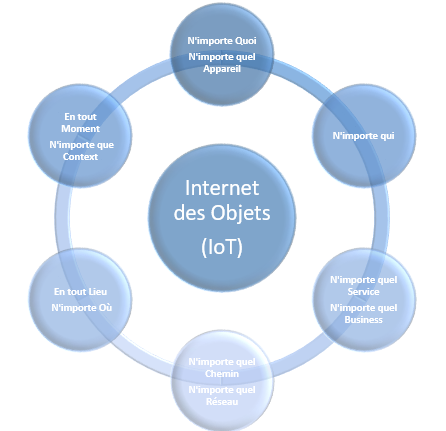
\includegraphics{IMAGES/ORIGINALS/Internet_des_Objets}
	\end{center}
	\caption{Internet des Objets}
\end{figure}

\textbf{L’Internet des Objets} peut être déf{\kern0pt}ini également comme « des données et des appareils disponibles en permanence à travers l’internet » \cite{hu2016security}.\\

\textbf{Un objet connecté} est un objet possédant la capacité d’échanger des données avec d’autres entités physiques ou numériques.\\

À peu près n'importe quel objet physique peut être transformé en un appareil IoT s'il peut être connecté à Internet pour être contrôlé ou communiquer des informations avec le réseau indépendamment de l’action humaine.\\

Pour illustrer, prenons un exemple dans le domaine de l’habitat intelligent, aussi connu sous le nom de Smart Home. Imaginez que votre réfrigérateur devienne intelligent. Un réfrigérateur capable de vous dire en temps réel le type de denrées qu’il y a à l’intérieur et capable de passer commande pour vous quand vous avez besoin de vous réapprovisionner.

Le réfrigérateur est un exemple typique mais le nombre d’objets qu’il est aujourd’hui possible de connecter pour s’échanger des données est illimité.\\

\begin{figure}[H]
	\begin{center}
		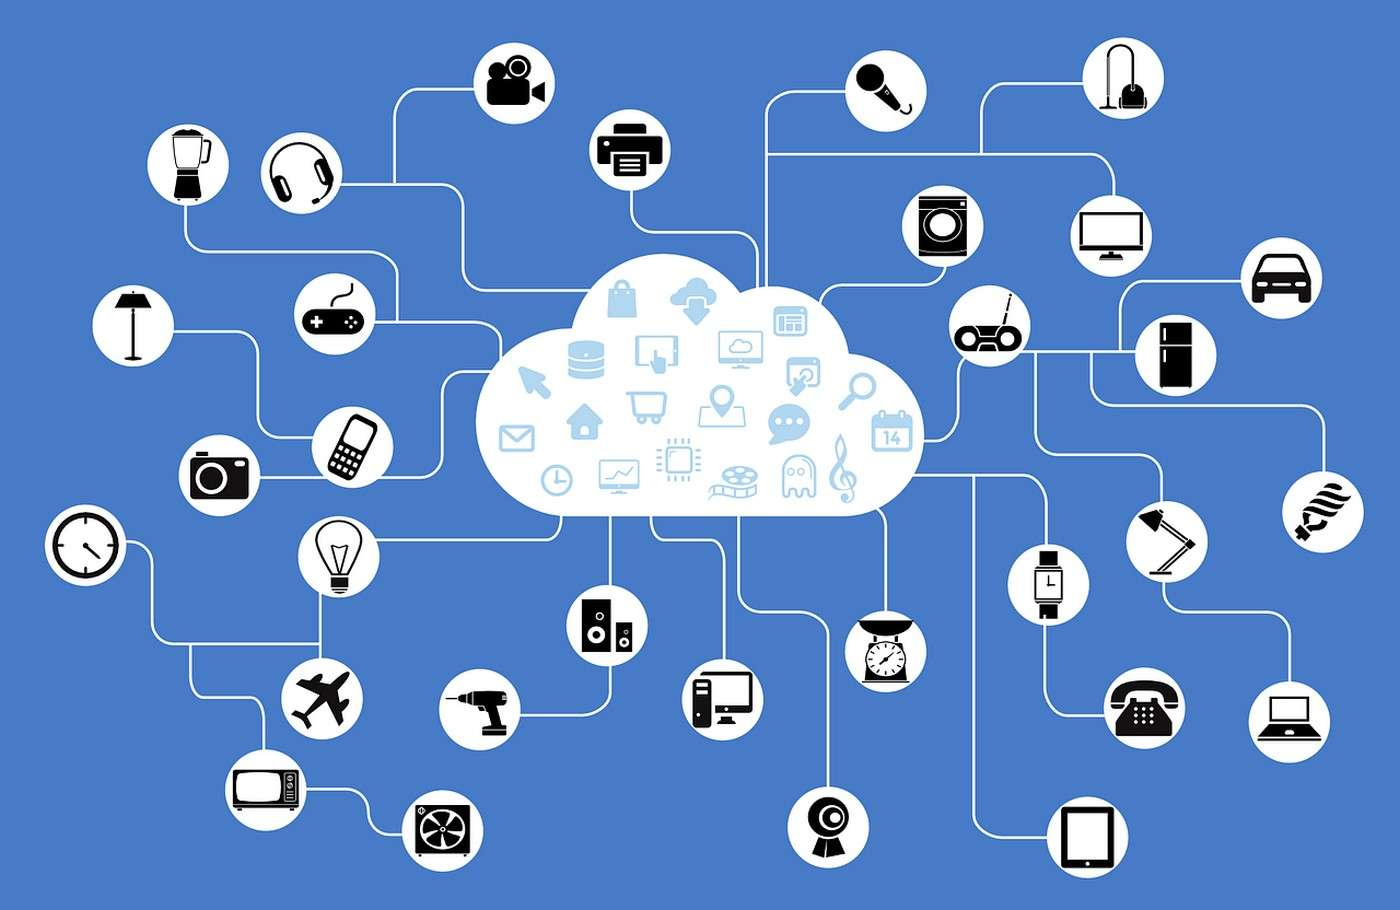
\includegraphics[width=16cm,height=14cm]{IMAGES/ORIGINALS/Internet_des_Objets_2}
	\end{center}
	\caption{Internet des Objets}
\end{figure}

\section{Caractéristiques}
Les caractéristiques fondamentales de l'IoT sont les suivantes \cite{patel2016iot,vermesan2014iot}:
\textbf{Inter connectivité}: en ce qui concerne l'IoT, tout peut être interconnecté avec l'infrastructure mondiale d'information et de communication.\\

\textbf{Services liés aux objets}: l'IoT est capable de fournir des services liés aux objets dans les limites des objets, tels que la protection de la vie privée et la cohérence sémantique entre les objets physiques et les objets virtuels associés. Af{\kern0pt}in de fournir des services liés aux objets dans les contraintes des objets, les technologies du monde physique et du monde de l'information vont changer.\\

\textbf{Hétérogénéité}: les appareils de l'IoT sont hétérogènes car basés sur dif{\kern0pt}férentes  plates-formes matérielles et réseaux. Ils peuvent interagir avec d'autres appareils ou plates-formes de services via dif{\kern0pt}férents réseaux.\\

\textbf{Changements dynamiques}: l'état des appareils change de manière dynamique, par exemple, le sommeil et le réveil, connectés et / ou déconnectés ainsi que le contexte des appareils, y compris l'emplacement et la vitesse. De plus, le nombre d'appareils peut changer dynamiquement.\\

\textbf{Échelle énorme}: le nombre d'appareils qui doivent être gérés et qui communiquent entre eux sera au moins d'un ordre de grandeur supérieur à celui des appareils connectés à l'Internet actuel. Encore plus critique sera la gestion des données générées et leur interprétation à des f{\kern0pt}ins d'application. Cela concerne la sémantique des données, ainsi que la gestion ef{\kern0pt}f{\kern0pt}icace des données.\\

\textbf{Sécurité}: à mesure que nous tirons parti de l'IoT, nous ne devons pas oublier la sécurité. En tant que créateurs et destinataires de l'IoT, nous devons concevoir pour la sécurité. Cela comprend la sécurité de nos données personnelles et la sécurité de notre bien-être physique. Sécuriser les points de terminaison, les réseaux et les données se déplaçant sur tout cela signif{\kern0pt}ie créer un paradigme de sécurité qui évoluera.\\

\textbf{Intelligence} : L'IoT est livré avec la combinaison d'algorithmes et de calcul, de logiciels et de matériel qui le rendent intelligent. Ce qui le rend encore plus intelligent, ce sont les données qu’il recueille à travers un capteur. L'intelligence ambiante dans l'IoT améliore ses capacités qui facilitent les choses pour répondre de manière intelligente à une situation particulière et les aide à ef{\kern0pt}fectuer des tâches spécif{\kern0pt}iques. Malgré toute la popularité des technologies intelligentes, l'intelligence dans l'IoT ne concerne que les moyens d'interaction entre les appareils, tandis que l'interaction utilisateur et appareil est obtenue par des méthodes d'entrée standard et une interface utilisateur graphique.\\

\textbf{Connectivité}: la connectivité permet l'accessibilité et la compatibilité du réseau. L'accessibilité se fait sur un réseau tandis que la compatibilité of{\kern0pt}fre la capacité commune de consommer et de produire des données.

\section{Architecture de l’IoT}	
L’IoT devrait être capable d’interconnecter des milliards d’objets hétérogènes via le réseau internet, ainsi il est judicieux d’adopter une architecture flexible. Le modèle de base est une architecture à trois-couches comportant les couches Application, Réseau, et Perception. D’autres modèles ont été proposé récemment qui ajoutent plus d’abstraction aux architectures des objets connectés. La f{\kern0pt}igure ci-dessous illustre les dif{\kern0pt}férentes catégories de l’architecture IoT \cite{al2015iot}.\\

\begin{figure}[H]
	\begin{center}
		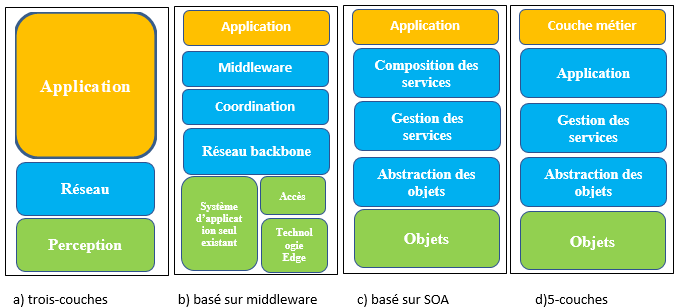
\includegraphics[width=\textwidth]{IMAGES/ORIGINALS/diverses_architectures_de_l'IoT}
	\end{center}
	\caption{Diverses architectures de l'IoT}
\end{figure}


\subsection{Architecture à trois couches}
\subsubsection{Couche perception }
La première couche de l’IoT, les Objets (appareils) ou couche perception, est un organe sensoriel de l’IoT, représente les capteurs physiques de l’IoT qui essaie de recueillir et traiter les données. Un capteur de température permet de traduire l’amplitude de la température en une tension électrique. Cette couche comprend principalement des éléments avec des étiquettes RFID, capteurs, et autre terminaux. Elle détecte les données de l’environnement. Certains facteurs sont pris en charge par la couche physique tels que : ressource, hétérogénéité, déploiement, protocoles.
\subsubsection{Couche réseau}
La couche réseau est chargée de récupérer les données collectées du capteur. L’échange des données se fait via cette couche. Ainsi, la couche réseau peut agréger les données dans sa propre base de données ou un stockage cloud.
\subsubsection{Couche application}
La couche application ou la couche interface utilisateur contient les méthodes d’interaction avec les applications de l’utilisateur.
\subsection{Architecture à cinq couches}
\subsubsection{Couche Objets}
La première couche de l’IoT, les Objets (appareils) ou couche perception, représente les capteurs physiques de l’IoT qui essaie de recueillir et traiter les données. Cette couche comprend les capteurs et les actionneurs qui fonctionnent dif{\kern0pt}féremment. Un capteur de température permet de traduire l’amplitude de la température en une tension électrique. On a d’autres grandeur mesurable tels que pression, luminosité, position, vitesse. Quant aux actionneurs, ils permettent d’agir dans le monde physique en changeant son état. Un actionneur peut allumer un appareil à distance. La couche perception collecte les informations du capteur, numérise et transmet les données à la couche Abstraction Objet via un canal sécurisé.
\subsubsection{Couche Abstraction Objet}
La couche Abstraction Objet transfert les données produit par la couche perception à la couche Gestion Service à travers des canaux sécurisés. Les données peuvent être transféré via des technologies variés tels que RFID, GSM(2G), UMTS(3G), LTE(4G), WI-FI, Bluetooth, Zigbee, etc. En plus, d’autres fonctions comme Cloud Computing et le traitement de gestion de données sont gérés par cette couche.
\subsubsection{Couche Gestion des Services}
La couche Gestion des Services garantit la fourniture des services en fonction de la demande de l'utilisateur dans un environnement réseau hétérogène.
\subsubsection{Couche Application}
La couche Application fournit les services demandés par les clients. Par exemple, la couche application peut fournir les mesures de température au client qui demande cette information.
Elle couvre dif{\kern0pt}férentes applications, à savoir: ville intelligente, transport intelligent, soins de santé, agriculture intelligente, maison intelligente, etc.
\subsubsection{Couche Business}
La couche métier(gestion) est chargée de gérer l’ensemble des activités et des services comme les modèles métiers. Elle aide à construire un graphique, un organigramme, un modèle métier, une prise de décision etc. basé sur les données reçues de la couche Application.
\section{Domaines d’application}
Il existe une panoplie de domaines d’application extrêmement diverses pour les secteurs de l’internet des objets, du machine to machine et des objets connectés. Parmi ces principaux domaines, nous citons : la smart city, la domotique, les transports, la santé, l’industrie, l’agriculture.
\begin{figure}[H]
	\begin{center}
		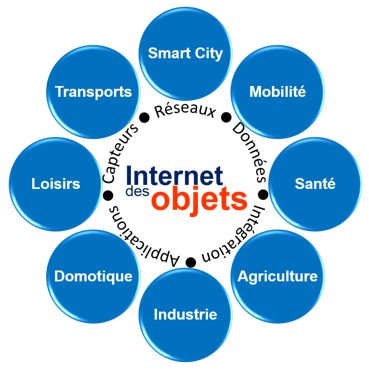
\includegraphics{IMAGES/ORIGINALS/Application_IoT}
	\end{center}
	\caption{Domaines d'application de l'IoT}
\end{figure}

\begin{enumerate}
	\item \textbf{Smart city}
	Dans les villes intelligentes, il améliore la qualité de vie des habitants en utilisant les nouvelles technologies pour accroître l’ef{\kern0pt}f{\kern0pt}icacité des services, optimiser l’éclairage, de maîtriser la consommation d’énergie et de réduire l’impact écologique des activités urbaines.
	\item \textbf{Domotique}
	La domotique regroupe l’ensemble des technologies permettant l’automatisation des équipements d’un habitat. Elle vise à apporter des solutions techniques pour répondre aux besoins de confort (gestion d’énergie, optimisation de l’éclairage et du chauf{\kern0pt}fage), de sécurité(alarme) et de communication (commandes à distance) \cite{locqueneux2015domotique}.
	La domotique couvre trois domaines principaux :
	\begin{enumerate}
		\item Confort de la vie quotidienne : l’IoT permettra aux propriétaires de villa de déclencher arrosage, fermeture des fenêtres ou tonte du gazon en fonction des informations transmises par les capteurs disposés dans le jardin.
		\item Assurer la protection des personnes et des biens par la prévention des risques d’accident (incendies, fuite de gaz, etc.).
		\item Faciliter les économies d’énergie grâce à la réaction maitrisée d’une maison intelligente.
	\end{enumerate}	
	\item \textbf{Santé}
	Dans le domaine de la santé, l’internet des objets of{\kern0pt}frira une sécurité accrue à un patient dont un capteur est intégré sur le corps qui donne la possibilité d’être monitoré à distance.
	Il peut informer un patient quand il est temps de prendre le médicament. En outre, cela pourrait éventuellement informer le médecin d’une situation d’urgence lui permettant ainsi de localiser le patient grâce à l’objet connecté.	
	\item \textbf{Transport}
	Des voitures connectées ou autonomes aux systèmes de transports intelligents, l’IoT pourra sauver des vies, réduire le traf{\kern0pt}ic et minimiser l’impact des véhicules sur l’environnement.
	
	\item \textbf{Industrie}
	Dans le secteur industriel, le machine to machine peut augmenter énormément la productivité et la performance d’une usine. Par exemple, supposons un réseau de capteurs polyvalents qui suit à distance et pilote le fonctionnement des machines en leur donnant la possibilité de déclencher elles-mêmes un réapprovisionnement en matières premières.	
	\item \textbf{Agriculture}
	L’internet des objets à un impact énorme sur le domaine de l’agriculture. Les éleveurs en bénéf{\kern0pt}icient en ef{\kern0pt}fectuant un suivi plus précis de l’alimentation, de la santé et de la sécurité du bétail. Ils peuvent aussi géolocaliser leur bétail en temps réel. Les agriculteurs peuvent aussi recueillir des données sur les engrais et les pesticides nécessaires à leurs cultures \cite{krigman2018agriculture}.
\end{enumerate}
\newpage
\section{Enjeux et déf{\kern0pt}is de l’IoT}
L’internet des objets soulève un nombre important de questions, mais le plus important porte certainement sur la sécurité. Beaucoup de produit connectés, dont certains que nous utilisons au quotidien af{\kern0pt}f{\kern0pt}ichent un réel manque de maturité impliquant de nouvelles préoccupation notamment autour de la conf{\kern0pt}identialité et la sécurité des données.
Mirai est un exemple type de cyberattaques résultant de menaces de sécurité liées à l’IoT.

\begin{table}[H]
	\begin{center}
		\begin{tabular}{|p{3cm}|p{10cm}|}
			\hline 
			\textbf{Enjeux} & \textbf{Déf{\kern0pt}is} \\ 
			\hline 
			Architecture & De nombreux chercheurs ont proposé diverses architectures non encore standardisé. \\ 
			\hline 
			Sécurité & L’échange d’information entre des milliards d’objets connecté sur internet se fait via une connexion réseau sans f{\kern0pt}il. \\ 
			\hline 
			Conf{\kern0pt}identialité & Les opérations d’accès aux prof{\kern0pt}ils entre objets sans interférences sont dif{\kern0pt}f{\kern0pt}iciles. \\ 
			\hline 
			Intéroperabilité & Communication machine à machine (M2M), un déf{\kern0pt}i de l’IoT dû à la nécessité de gérer un grand nombre d’objets hétérogènes qui appartiennent à dif{\kern0pt}férentes plates-formes. \\ 
			\hline 
			Disponibilité & La capacité à fournir des services à tout moment, n’importe où et n’importe quoi est un déf{\kern0pt}is. \\ 
			\hline 
			Mobilité & L'utilisateur ou les appareils qui se connectent peuvent obtenir les services lors de leurs déplacements, ce qui constitue un déf{\kern0pt}i. \\ 
			\hline 
			Scalabilité & La possibilité d'ajouter de nouveaux appareils qui n'af{\kern0pt}fecte pas la qualité de services existent est un déf{\kern0pt}i. \\ 
			\hline 
		\end{tabular} 
	\end{center}
	\caption{Enjeux et déf{\kern0pt}is de l'IoT}
\end{table}

 \section{Sécurité, conf{\kern0pt}identialité (privacy) en IoT}
 L’IoT nécessite cinq phases, de la collecte des données, du stockage, du traitement, de la transmission des données à la livraison des données aux utilisateurs f{\kern0pt}inaux sur demande ou non \cite{hu2016security}. Les capteurs collectent dans de nombreux cas des données extrêmement sensible (personnelles). En ef{\kern0pt}fet les objets connectés produisent de grandes quantités de données à la phase de collecte de données et le traitement de cette masse de données implique de nouvelles préoccupations notamment autour de la conf{\kern0pt}identialité et la sécurité des données. 
\begin{figure}[H]
	\begin{center}
		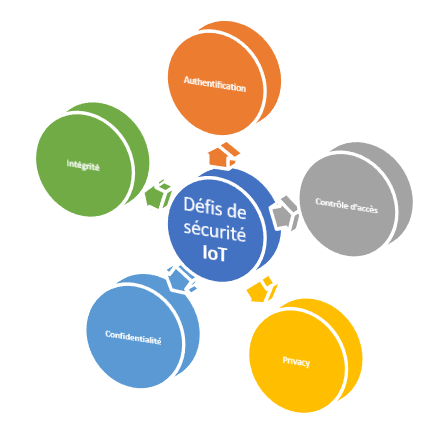
\includegraphics[width=0.7\textwidth]{IMAGES/ORIGINALS/DsIoT}
	\end{center}
	\caption{Déf{\kern0pt}is de sécurité IoT}
\end{figure}

\subsection{Sécurité pour l’IoT}
La sécurité est l’af{\kern0pt}faire de tous, elle concerne chacun de nous. Si vous achetez un verrou « intelligent » pour votre porte d’entrée, il est fort probable que vous allez vous faire pirater dans un premier temps puis cambrioler. L’IoT a des avantages et apporte tous celui d’internet à des éléments comme les thermostats et les ampoules par exemple mais sans oublier qu’il apporte également les problèmes d’internet. A présent que les gens ont leur réfrigérateurs, sonnettes, télévisions, ampoules, caméras de sécurité, haut-parleur connectés au Wi-Fi, presque tous les appareils de la maison peuvent être compromis ou rendu inutiles. En ef{\kern0pt}fet les objets connectés peuvent servir de point d’accès à votre réseau avec vos portables, votre PC, bref toute votre vie.


La menace qui pèse sur les appareils connectés à Internet ne vient pas uniquement du fait qu’ils sont connectés à Internet, mais aussi parce que les fabricants d’appareils n’ont pas toujours conçu leurs produits en privilégiant la sécurité. À mesure que l'IoT se répand largement, les cyberattaques risquent de devenir de plus en plus physiques (et pas simplement virtuelles) \cite{clearfield2013rethinkingsiot}. Les appareils contrôlés par ordinateur dans les automobiles, tels que les freins, les moteurs, les serrures, les klaxons, les systèmes de chauf{\kern0pt}fage et les tableaux de bord, se sont révélés vulnérables aux attaquants qui ont accès au réseau de bord \cite{andy2013hackers,boyle2010proof}. La possibilité qu'un intrus puisse démarrer à distance le chauf{\kern0pt}fage, régler le climatiseur, déverrouiller les portes, déployer des airbags pendant que vous conduisez sans accident ou tourner le volant d'une voiture en marche est en ef{\kern0pt}fet inquiétante, ef{\kern0pt}frayante.


Jusque-là l’essentiel des dommages subit par l’IoT a été causé par les botnets. En septembre 2016, une attaque a été mis en place par des centaines de milliers d’objets connecté piraté pour former un énorme botnet appelé Mirai. Ce malware a exploité des vulnérabilités (que les fabricants d’objet connecté ne prenaient pas en compte) dans plus de 600 000 appareils IoT pour créer une attaque massive par déni de service distribué (\textbf{DDoS}). Il avait pour objectif de dénoncer les risques de l’IoT.


En raison de la vulnérabilité du WPA2(protocole qui sécurise les échanges en Wi-Fi), tout ce qui est connecté à un réseau Wi-Fi risque d’être piraté \cite{kasperski201krack}. L'année suivante après Mirai, une attaque appelée KRACK acronyme de Key Reinstallation Attack (attaque de réinstallation de clé) a infecté presque tous les appareils connectés à Internet connectés au Wi-Fi. L'attaque était paralysante et dif{\kern0pt}f{\kern0pt}icile à résister, en partie parce que l'Internet des objets fonctionne sur de nombreux systèmes d'exploitation essentiellement dif{\kern0pt}férent. Lorsqu'un téléphone ou un ordinateur est touché par un virus, les fabricants de logiciels sont généralement prompts à émettre un correctif. Mais des choses comme les routeurs ou les sonnettes connectées à Internet ne sont pas mis à jour aussi régulièrement que les systèmes d’exploitation informatique pour se protéger contre les vulnérabilités, et beaucoup d'entre elles n'ont pas été construites avec le même type de protocoles de sécurité que les ordinateurs \cite{pardes2020iot}. C’est une réalité, l’IoT nous rend encore plus connecter et cette connexion de tous les instants vient avec son l’eau de risque qu’on ne peut pas ignorer. Les menaces virtuelles vont s’immiscer dans le monde physique, ce qui signif{\kern0pt}ie que le piratage des appareils peut avoir des conséquences dangereuses dans le monde réel.


L'IoT n'est pas encore arrivé à maturité et est extrêmement vulnérable à toutes sortes de menaces et d'attaques ou vol de données. Les systèmes de prévention ou de récupération utilisés dans le réseau traditionnel et Internet ne peuvent pas être utilisés dans l'IoT en raison de sa connectivité \cite{hu2016security}. Les raisons de sa vulnérabilité sont multiples \cite{atzori2010iot}. Primo, souvent ses composants passent la plupart du temps sans surveillance; et ainsi, il est facile de les attaquer physiquement. Secundo, la plupart des communications sont sans f{\kern0pt}il, ce qui rend l'écoute extrêmement simple. Enf{\kern0pt}in, la plupart des composants IoT sont caractérisés par de faibles capacités en termes à la fois d'énergie et de ressources informatiques (c'est particulièrement le cas pour les composants passifs) et, par conséquent, ils ne peuvent pas mettre en œuvre des schémas complexes prenant en charge la sécurité.


La sécurité des informations et du réseau doit être dotée de propriétés telles que, la conf{\kern0pt}identialité, l'intégrité, l'identif{\kern0pt}ication et la disponibilité. Plus précisément, les problèmes majeurs de l’IoT liés à la sécurité concernent l'\textit{authentif{\kern0pt}ication} et l'\textit{intégrité des données} \cite{atzori2010iot} : 
\begin{itemize}
	\item[$\bullet$] L'authentif{\kern0pt}ication est requise pour établir une connexion entre les appareils et l'échange de nombre de clés publiques et privées via le nœud pour empêcher le vol de données. L'authentif{\kern0pt}ication est dif{\kern0pt}f{\kern0pt}icile car elle nécessite généralement des infrastructures d'authentif{\kern0pt}ication et des serveurs appropriés qui atteignent leur objectif grâce à l'échange de messages appropriés avec d'autres nœuds. Dans l'IoT, de telles approches ne sont pas réalisables étant donné que les étiquettes RFID passives ne peuvent pas échanger trop de messages avec les serveurs d'authentif{\kern0pt}ication. Le même raisonnement s'applique (de manière moins restrictive) aux nœuds de capteur également.	
	\item[$\bullet$] Les solutions d'intégrité des données doivent garantir qu'un adversaire ne peut pas modif{\kern0pt}ier les données de la transaction sans que le système détecte le changement. En d’autre terme, elles garantissent que les données qui sont arrivées au nœud récepteur sont inchangées et restent telles que transmises par la source (expéditeur). Un autre facteur critique qui influence l'intégrité des données est la robustesse et les capacités de tolérance aux pannes du système IoT. Les réseaux de capteurs, tels que les solutions RFID, sont également confrontés à d'autres problèmes qui limitent leur capacité à surmonter les problèmes d'intégrité, car bon nombre de leurs composants passent la plupart du temps sans être pris en charge, sans surveillance \cite{musonda2018iot}. Les données peuvent être modif{\kern0pt}iées par des attaquants pendant qu'elles sont stockées dans le nœud ou lorsqu'elles traversent le réseau \cite{karygiannis2007guidelines}. Pour protéger les données contre ces types d'attaque, les protections en lecture et en écriture ainsi que les méthodes d'authentif{\kern0pt}ication sont généralement des solutions courantes à ces problèmes. Les ressources trouvées dans les systèmes IoT courants ne prennent pas en charge les techniques cryptographiques (permettant de stocker, traiter et partager des données protégées sans que le contenu de l'information soit accessible à d'autres parties) typiques en raison des ressources limitées disponibles \cite{musonda2018iot}. L'intégrité de l'Internet des objets doit non seulement être protégée des sources externes mais également des processus internes, tels que l'intégrité des services.
\end{itemize}


\subsection{Conf{\kern0pt}identialité pour l’IoT}
Il y a ensuite la question de la conf{\kern0pt}identialité. La conf{\kern0pt}identialité des données est une condition pour que les données ne soient disponibles que pour les utilisateurs autorisés. Elle consiste à garder les données privées plutôt que de les autoriser à être disponibles dans le domaine public.


L’IoT représente un environnement dans lequel la vie privée des individus est fortement menacée. Si des caméras et des microphones sont installés autour de votre maison, ils vous regardent et vous écoutent. Tout dans l'internet des objets collecte des données et toutes ces données sont d’une valeur inestimable. Ainsi, lorsque les entreprises gagneront de l'argent en vous vendant des objets connectés intelligents en premier lieu, leur modèle commercial IoT implique probablement la vente d'au moins certaines de ces données également.


Ce qui arrive à ces données est une question de conf{\kern0pt}identialité d'une importance vitale. Toutes les entreprises de maisons intelligentes ne construisent pas leur modèle commercial autour de la collecte et de la vente de vos données, mais certaines le font \cite{ranger2020iot}.


De nombreux appareils de dernière génération dans nos maisons sont équipés d'une connectivité qui permet une grande commodité, mais cet avantage a un prix (des risques potentiels d'espionnage et de sécurité). En janvier 2014, Forbes a répertorié de nombreux appareils connectés à Internet tels que des téléviseurs, des appareils de cuisine, des modems(et ISP), des, des caméras, des thermostats(chauf{\kern0pt}fage et climatisation), et des équipements de buanderie qui peuvent déjà « espionner des personnes dans leur propre maison » \cite{steinberg2014spying}. Cela signif{\kern0pt}ie que les détails les plus f{\kern0pt}ins de votre vie personnelle, tels que exposés par votre réfrigérateur intelligent, votre télévision intelligent ou votre haut-parleur intelligent, peuvent être recueillis et vendus à quelqu'un d'autre ou pour faire du chantage. Google et Apple ont tous deux admis, l'an dernier, que les enregistrements capturés par leurs haut-parleurs intelligents étaient examinés par des entrepreneurs, y compris des extraits audio maladroits et intimes.


La sécurisation des échanges de données est nécessaire pour éviter de perdre ou de compromettre la conf{\kern0pt}identialité.
\section{Conclusion}{
L’IoT est un concept en évolution constante dont l’objectif est d’étendre le réseau internet en interconnectant les objets connectés, ainsi ef{\kern0pt}fectué des échanges de données aux objets du monde physique. Ces objets connectés à internet peuvent prendre la forme de n’importe quel objet du quotidien.


Il existe plusieurs architectures de l’IoT tels que l’architecture basé trois-couches, basé sur middleware, basé sur SOA et basé cinq-couches. Tout appareil connecté à Internet présente un risque élevé, et les appareils IoT ne font pas exception. L’IoT peut être vu comme « Interconnections of Threats » c’est-à-dire interconnexions des menaces dû à l’extension du réseau internet. La sécurité et la conf{\kern0pt}identialité des données sont de grands déf{\kern0pt}is dans l’IoT. Lors de la transmission transparente des données, il est important de se cacher des appareils d'observation sur Internet qui sont susceptibles de nous espionner.
		
		
		%\chapter{Attaques DDoS} 
\section{Introduction}
	Une fois qu’un service est accessible via internet, il faut pouvoir estimer le risque de déni de service distribué. Un risque qui doit pas être laissé de côté, pouvant toucher directement à la disponibilité des ressources et qui peut être frustrant et coûteux aux entreprises. Un déni de service apparaît probablement lorsqu’il y a une surcharge des composants individuels du système d’information. Si cela est provoqué délibérément par une source externe, on parle alors d’attaque DoS, en l’occurrence, le remplissage d’un canal de communication ou une zone de stockage jusqu’à ce qu’on ne puisse plus l’utiliser.\\

Une méthode particulièrement efficace est lorsque le système est inondé de trafics illégitimes provenant de centaines, de milliers, voire de millions d’autres ordinateurs (souvent compromis). Ceci est connu sous le nom d’attaque DDoS.\\

Dans ce chapitre, nous exposons les attaques DDoS, en passant en revue son fonctionnement, les différentes catégories d’attaque, les motivations derrières les attaques DDoS et ainsi que quelques mesures de prévention.


	\section{Définition d’attaque DDoS}
	Une attaque par déni de service distribué (DDoS pour Distributed Denial of Service en anglais) est une tentative malveillante de perturber le trafic normal d'un serveur, d'un service ou d'un réseau ciblé en submergeant la cible ou son infrastructure environnante par un flot de trafic Internet. Les attaques DDoS atteignent leur efficacité en utilisant plusieurs systèmes informatiques compromis comme sources de trafic d'attaque. Les machines exploitées peuvent inclure des ordinateurs et d'autres ressources en réseau telles que les appareils IoT. Par analogie, une attaque DDoS est comme un embouteillage obstruant l'autoroute, empêchant le trafic régulier d'arriver à sa destination souhaitée\cite{cloudflareddos}.\\

D’un point de vue technique, le terme déni de service est utilisé pour parler de l’incapacité du service à répondre aux trafics légitime durant l’attaque.\\

	\begin{figure}[ht]
		\begin{center}
			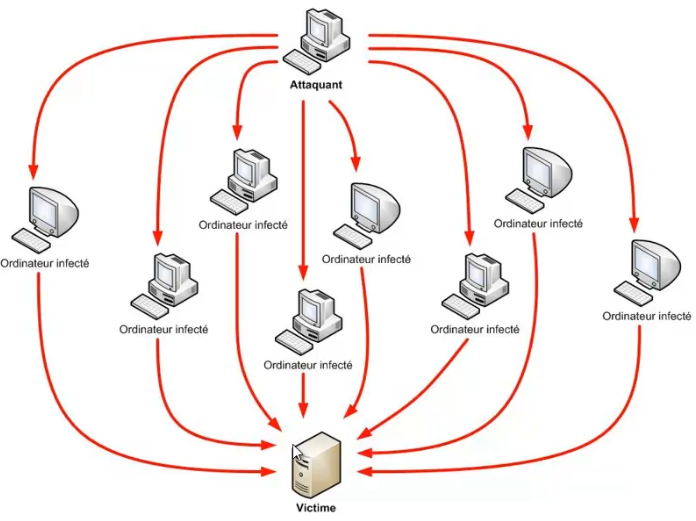
\includegraphics[width=\textwidth]{IMAGES/ORIGINALS/Architecture_attaque_DDoS}
		\end{center}
		\caption{Architecture d'attaque DDoS}
	\end{figure}

	\pagebreak
	\section{Principe de fonctionnement des attaques DDoS}
	Une attaque DDoS implique pour un attaquant de prendre le contrôle d'un réseau de machines en ligne afin de mener une attaque. Les ordinateurs et autres machines (comme les appareils IoT) sont infectés par un malware, qui les transforme en bots (ou zombies). Le pirate contrôle alors à distance le groupe de bots, appelé un botnet.\\
	
	Un Botnet est une contraction des termes « robot » et « network » où chaque appareil infecté est appelé bot. Il fait référence à un groupe d'ordinateurs qui ont été infectés par des logiciels malveillants et qui sont tombés sous le contrôle d'un attaquant. Les botnets peuvent être conçus pour accomplir des tâches illégales ou malveillantes, notamment l'envoi de spam, le vol de données, les ransomwares, les clics frauduleux sur les publicités ou les attaques par déni de service distribué (DDoS).\\
	
	Une fois qu'un botnet a été mis en place, l'attaquant est en mesure de diriger les machines en envoyant des instructions mises à jour à chaque bot via une méthode de contrôle à distance. Quand l’adresse IP d'une victime est ciblée par le botnet, chaque bot répond en envoyant des requêtes à la cible, ce qui peut saturer le serveur ou le réseau ciblé, entraînant un DoS pour le trafic normal. Étant donné que chaque bot est un périphérique Internet légitime, il peut être difficile de séparer le trafic d'attaque du trafic normal \cite{cloudflareddos}.


	\section{Catégories d’attaque DDoS}	
	Le nombre d’attaques par déni de service distribué s’est considérablement élevé au cours des dernières années. Ces attaques sont aujourd’hui fréquentes, et peuvent viser toute entité disposant d’un système d’information ou d’une infrastructure réseau connectée à Internet.\\
	
	Les botnets ciblent des vulnérabilités dans différentes couches d’interconnexion des systèmes ouverts et un vecteur d’attaque peut généralement être classé dans l’une des trois grandes catégories suivantes \cite{netscoutddos} : attaques par déni de service volumétriques, attaques par déni de service d’épuisement d’états TCP (TCP state-exhaustion attacks), et attaque de la couche d’application.

	\subsection{Attaques de la couche d’application}
	Généralement appelées attaques DDoS de couche 7 (en référence à la 7e couche du modèle OSI), le but est d'épuiser les ressources de la cible. Les attaques ciblent la couche où les pages Web sont générées sur le serveur et livrées en réponse aux requêtes HTTP. Une seule requête HTTP est peu coûteuse à exécuter côté client et peut coûter cher au serveur cible de répondre car le serveur doit souvent charger plusieurs fichiers et exécuter des requêtes de base de données afin de créer une page Web. Ces attaques sont souvent difficiles à empêcher car le trafic peut être difficile à détecter comme malveillant.\\
	La prolifération des dispositifs IoT non sécurisés au cours des dernières années a été avantageux pour les attaquants DDoS car il existe désormais un nombre presque illimité de dispositifs intelligents qui peuvent être utilisés comme botnet pour lancer des attaques de couche application plus avancées.

	\subsubsection{HTTP Flood}
	\begin{figure}[h]
		\begin{center}
			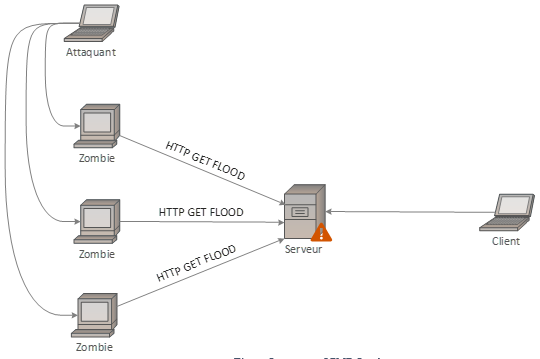
\includegraphics[width=\textwidth]{IMAGES/ORIGINALS/Attaque_HTTP_Flood}
		\end{center}
		\caption{Attaque HTTP Flood}
	\end{figure}

	Dans une attaque DDoS HTTP Flood, l'attaquant exploite des requêtes HTTP POST ou GET généralement légitimes pour attaquer une application ou un serveur Web. Les HTTP Flood n'utilisent pas de paquets malformés, de techniques de réflexion, ou d'usurpation et nécessitent moins de bande passante que les autres attaques pour faire tomber le serveur ou le site ciblé. L'attaque est plus efficace lorsqu'elle oblige le serveur ou l'application à allouer le maximum de ressources possible en réponse à chaque requête.
	
	\subsubsection{Slowloris}
	C’est un outil d’attaque écrit en Perl, créé par RSnake (Robert Hansen), une attaque de type DoS hautement ciblée, permettant à une machine de faire tomber un serveur en épuisant les ressources de connexion notamment des serveurs web sans affecter les autres services ou ports du réseau cible. Il y parvient en maintenant ouverts autant de connexions au serveur Web cible que possible. Il accomplit cela en créant des connexions au serveur cible, mais en n'envoyant qu'une demande partielle. Slowloris envoie constamment plus d'en-têtes HTTP, mais ne termine jamais une demande. Le serveur ciblé garde ouverte chacune de ces fausses connexions. Cela déborde finalement le pool de connexions simultanées maximum et conduit au refus de connexions supplémentaires de clients légitimes.\\
	
	Lorsque de nombreux hôtes malveillants lancent simultanément des attaques Slowloris depuis un botnet, toutes les connexions disponibles vers un serveur cible sont ouvertes en même temps. Par conséquent, le serveur ne peut pas gérer les requêtes HTTP légitimes.

	\subsubsection{Imitation de la navigation des utilisateurs}
	Les botnets sont devenus de nos jours les principaux moteurs des activités malveillantes dans le cyberespace. Pour soutenir leurs réseaux de botnet et masquer leurs actions malveillantes, les détenteurs de ces réseaux imitent des cyber-comportements légitimes pour passer inaperçus. Le but de ces attaques est de submerger le site Web cible avec un volume suffisamment élevé des botnets, rendant ainsi impossible le trafic légitime ou le plantage du site.
Le motif commun derrière de telles attaques DDoS peut être financier ou politique.\\

	Une méthode courante utilisée pour empêcher ce type d'attaque consiste à utiliser une sorte de contrôles captcha, affichant des images ou des modèles auxquels un humain est capable de répondre, mais un bot aurait du mal à le faire.

	\subsection{Attaques d'épuisement d'état TCP}
	Les attaques protocolaires, également appelées attaques d'épuisement d'état (state-exhaustion attack), provoquent une interruption de service en consommant toute la capacité des tables d'état disponible des serveurs d'applications Web ou des ressources intermédiaires comme les pare-feu et les répartiteurs de charge. Les attaques protocolaires utilisent les faiblesses des couches 3 et 4 de la pile de protocoles pour rendre la cible inaccessible.
Ces attaques sont généralement utilisées par des attaquants déterminés qui surveillent et ajustent leurs attaques pour un impact maximal.\\
	
	Les attaques courantes d'épuisement d'état peuvent inclure: SYN Flood, SSL/TLS Exhaustion, DNS Flood, attaque Smurf (dans le cadre du protocole ICMP).

	\subsubsection{SYN Flood}
	\begin{figure}[h]
		\begin{center}
			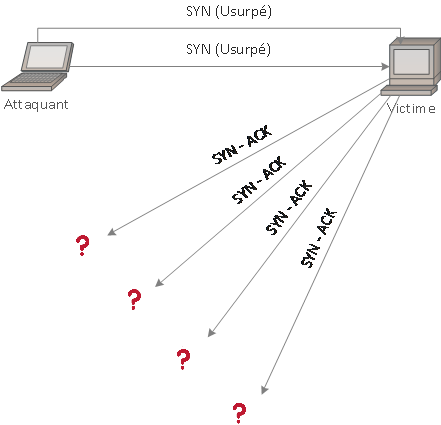
\includegraphics[width=\textwidth]{IMAGES/ORIGINALS/Attaque_SYN_Flood}
		\end{center}
		\caption{Attaque SYN Flood}
	\end{figure}
	
	Une attaque DDoS SYN flood exploite une faiblesse connue de la séquence de connexion TCP (the « Three-Way Handshake »), dans laquelle une demande SYN pour établir une connexion TCP avec un hôte doit être répondue par une réponse SYN-ACK de cet hôte, et puis confirmé par une réponse ACK du demandeur. Dans un scénario SYN Flood, le demandeur envoie plusieurs demandes SYN à partir d'une adresse IP usurpée, qui ne peut pas répondre à la requête SYN-ACK de l'hôte. Le système hôte continue d'attendre l'accusé de réception pour chacune des demandes, liant les ressources jusqu'à ce qu'aucune nouvelle connexion ne puisse être établie, et entraînant finalement un déni de service.

	\subsubsection{Attaque Smurf}
	\begin{figure}[h]
		\begin{center}
			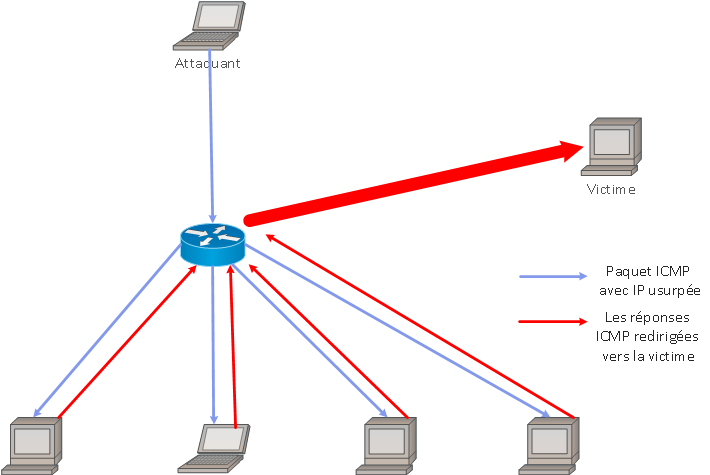
\includegraphics[width=\textwidth]{IMAGES/ORIGINALS/Attaque_Smurf}
		\end{center}
		\caption{Attaque Smurf}
	\end{figure}
		
	Le nom Smurf vient du code source de l'outil d'exploitation original, smurf.c, créé par un individu appelé TFreak en 1997 \cite{ciscoguideagainstddos}. 
Les attaques de Smurf sont quelque peu similaires aux ICMP Flood, car les deux sont effectuées en envoyant une flopée de paquets de demande d'écho ICMP.
Contrairement à ICMP Flood régulière, Smurf est un vecteur d'attaque d'amplification qui augmente son potentiel de dégâts en exploitant les caractéristiques des réseaux de diffusion.\\

	Dans une attaque smurf, un attaquant diffuse un grand nombre de paquets ICMP avec l'adresse IP source usurpée de la victime vers un réseau utilisant une adresse de diffusion IP. Cela oblige les périphériques du réseau à répondre en envoyant une réponse à l'adresse IP source.
	
	\pagebreak
	\subsubsection{DNS Flood}
	\begin{figure}[h]
		\begin{center}
			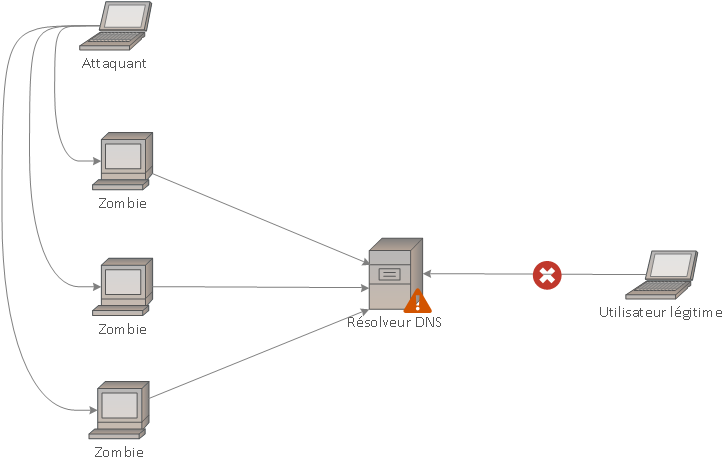
\includegraphics[width=\textwidth]{IMAGES/ORIGINALS/Attaque_DNS_Flood}
		\end{center}
		\caption{Attaque DNS Flood}
	\end{figure}

	Un DNS Flood est un type d'attaque DDoS où un attaquant submerge les serveurs DNS d'un domaine particulier dans le but de perturber la résolution DNS de ce domaine. Si un utilisateur n'est pas en mesure de trouver le répertoire, il ne peut pas rechercher l'adresse afin d'effectuer l'appel pour une ressource particulière. En perturbant la résolution DNS, une attaque par inondation DNS compromettra la capacité d'un site Web, d'une API ou d'une application Web à répondre au trafic légitime.\\

	Les attaques par inondation DNS utilisent les connexions à large bande passante des caméras IP, d'autres appareils IoT pour submerger directement les serveurs DNS des principaux fournisseurs. Le volume de demandes des appareils IoT submerge les services du fournisseur DNS et empêche les utilisateurs légitimes d'accéder aux serveurs DNS du fournisseur.\\

	Ces attaques DNS diffèrent des attaques par amplification DNS. Contrairement aux inondations DNS, les attaques d'amplification DNS reflètent et amplifient le trafic des serveurs DNS non sécurisés afin de masquer l'origine de l'attaque et d'augmenter son efficacité.

	
	\pagebreak
	\subsection{Attaques volumétriques}
	L’inaccessibilité d’une machine peut être réalisé en surchargeant la bande passante avec des volumes significativement élevés de trafic malveillant. Les attaques DoS et DDoS ciblent directement les réseaux ainsi que leurs périphériques de connexion. Un routeur ne peut traiter qu’une certaine quantité de données à la fois, si cette capacité est dépassée en raison notamment d’une attaque, les services correspondants ne seront alors plus fonctionnels pour les autres utilisateurs.
Les attaques volumétriques sont généralement lancées contre une cible spécifique, généralement des services critiques de fournisseur de services (SP) ou des clients d'entreprise. Les modèles d’attaque sont principalement : ICMP Flood, UDP Flood, IPSec Flood, IP/ICMP Fragmentation, attaques d’amplification de réflexion. 

	\subsubsection{UDP Flood}
	Une UDP Flood est une forme d'attaque volumétrique par déni de service (DoS). Par définition, c’est toute attaque DDoS qui attaque une cible avec des paquets UDP (ne nécessitant pas d’établissement de connexion préalable ou de session). Le but de l'attaque est d'inonder des ports aléatoires sur un hôte distant. Cela oblige l'hôte à vérifier à plusieurs reprises l'application qui écoute sur ce port et (lorsqu'aucune application n'est trouvée) répond avec un paquet ICMP « Destination inaccessible »\cite{impervaddos}. Ce qui conduit à l’inaccessibilité.\\

	Lorsque des attaques par UPD Flood émanent de plusieurs machines, l'attaque est considérée comme une menace de déni de service distribué (DDoS).

	\subsubsection{ICMP Flood}	
	\begin{figure}[h]
		\begin{center}
			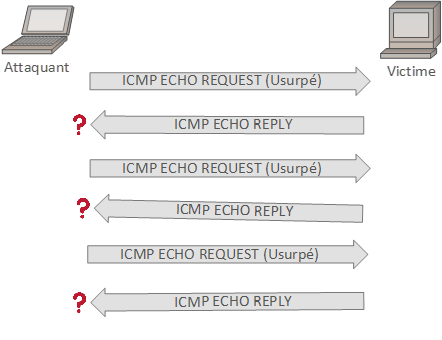
\includegraphics[width=\textwidth]{IMAGES/ORIGINALS/Attaque_ICMP_Flood}
		\end{center}
		\caption{Attaque ICMP Flood}
	\end{figure}
		
	Similaire en principe à l'attaque UDP Flood, une ICMP Flood submerge la ressource cible avec des paquets de requête d'écho ICMP (ping), envoyant généralement des paquets le plus rapidement possible sans attendre de réponses. Généralement, les messages de demande d'écho et de réponse d'écho ICMP sont utilisés pour envoyer une requête ping à un périphérique réseau afin de diagnostiquer l'intégrité et la connectivité du périphérique et la connexion entre l'expéditeur et le périphérique.\\
	
	Ce type d'attaque peut consommer de la bande passante sortante et entrante, car les serveurs de la victime tentent souvent de répondre avec des paquets de réponse d'écho ICMP, ce qui entraîne un ralentissement global significatif du système. Cette attaque peut être réalisé à l’aide d’outils personnalisé ou code tels que hping and scapy. Elle nécessite au préalable la connaissance de l’adresse IP de la cible.

	\subsubsection{Fragmentation IP/ICMP}
	Une attaque par fragmentation IP/ICMP (soit Internet Protocol / Internet Control Message Protocol) est une forme courante d'attaque volumétrique par déni de service (DoS). Dans une telle attaque, les mécanismes de fragmentation des datagrammes sont utilisés pour submerger le réseau.\\

	Le processus de fragmentation IP est un processus de communication dans laquelle les datagrammes IP sont décomposés en petits paquets, transmis sur un réseau puis réassemblés dans le datagramme d'origine.\\

	La fragmentation est indispensable pour la transmission des données, puisque chaque réseau a une limite unique en matière de taille de datagrammes qu'il peut traiter, qu’on appelle unité de transmission maximale (Maximum Transmission Unit soit MTU). Si le datagramme envoyé est plus grand que le MTU du serveur de réception, il doit être fragmenté pour être transmis complètement.\\

	Dans le cas d’une attaque DoS, l'attaquant peut utiliser la fragmentation IP pour cibler les systèmes de communication, ainsi que les composants de sécurité. Les attaques de fragmentation basées sur ICMP soumettent généralement de faux fragments qui ne peuvent pas être défragmentés. Cela entraîne à son tour le placement des fragments dans un stockage temporaire, occupant de la mémoire et dans certains cas épuisant toutes les ressources de mémoire disponibles.\\

	\subsubsection{Amplification DNS}
	\begin{figure}[hp]
		\begin{center}
			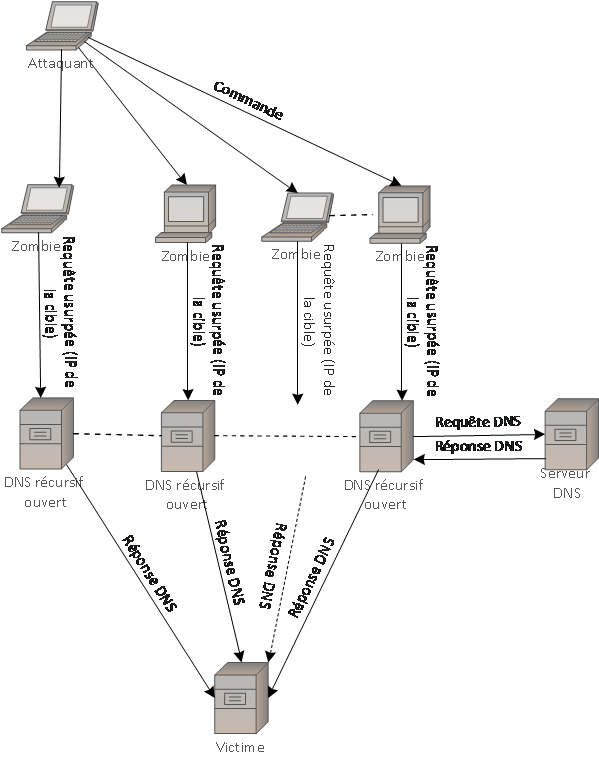
\includegraphics[width=\textwidth]{IMAGES/ORIGINALS/Amplification_DNS}
		\end{center}
		\caption{Architecture d'attaque par amplification DNS}
	\end{figure}	
			
	Les attaques par amplification DNS renforcent la force des attaques de DDoS. Plutôt que d’envoyer le trafic directement d’un botnet à une victime, le botnet envoi des demandes à d’autres systèmes. Ces systèmes répondent en envoyant des volumes de trafic plus importants à la victime. La figure 7 est une illustration de ce type d’attaque.
		
	
	\subsection{Attaques Zero-day}
La définition « Zero-day » englobe toutes les attaques inconnues ou nouvelles, exploitant des vulnérabilités pour lesquelles aucun correctif n'a encore été publié.
En général, le terme attaque Zero-Day (ou attaque 0-day) est utilisé pour les attaques qui utilisent de nouvelles vulnérabilités de sécurité logicielle, dont la communauté n'est pas encore au courant. Cela peut prendre un certain temps entre le moment où le malfaiteur détecte la vulnérabilité et la publication et l'installation du nouveau patch (correctif). Pendant tout ce temps, la vulnérabilité sera activement utilisée pour bloquer les ressources et voler des informations.\\ 

	Par exemple, pour organiser une attaque DDoS réussie, le pirate informatique doit mettre en place un réseau de zombie en peu de temps. La tactique de vulnérabilité Zero-Day est un choix parfait à cet effet. Par conséquent, cette approche gagne en popularité auprès des pirates du monde entier. Pour atteindre leur objectif, les malfaiteurs doivent accéder à un serveur qui exécute un logiciel avec une vulnérabilité de Zero-day. Le serveur peut alors être utilisé pour ce type d'attaques. Cela signifie également qu'il n'est pas nécessaire d'utiliser un grand nombre de machines compromises.\\

	Le terme zero-day est bien connu des membres de la communauté des pirates informatiques, où la pratique du trading de vulnérabilités zero-day est devenue une activité populaire.

	
	\section{Motivations}
	Les attaques DDoS deviennent rapidement le type de cyber-menace le plus répandu. Étant donnée la facilité de mises en place des attaques DDoS à faible coût avec très peu de préparation, il est devenu clair que toute organisation court le risque de subir une attaque à tout moment. Mais qu’est-ce qui peut motiver l’auteur d’une attaque ? 
Voici quelques-unes des raisons\cite{bellitddos}.

	\subsection{Cyberactivisme}
	Le Cyberactivisme, soit en anglais (Hacktivism). Le DDoS peut servir souvent un mode de protestation contre les sociétés et les gouvernements dont les actions sont considérées comme « incorrectes » ou « mauvaises » par l’attaquant. Par exemple des attaques par des groupes comme Anonymous contre des organisations telles que l’État islamique et le FBI) au personnel et au mesquin (comme des serveurs de jeux informatiques en ligne mis en panne par des joueurs irrités au sujet de changements récents apportés au jeu).

	\subsection{Vandalisme}
	Parfois des attaquants mettent un site Web en panne simplement pour prouver qu’il est possible de le faire, ou pour nulle autre raison que de « se faire remarquer » par une communauté d’utilisateurs en ligne. On attribue ces types d’attaques à ce qu’il est convenu d’appeler des « pirates adolescents » (script kiddies en anglais), en raison de la puérilité des motifs.

	\subsection{Concurrence}
	Si le site Web d’une entreprise donnée tombe en panne, c’est une bonne nouvelle pour ses concurrents. L’entreprise touchée perdra non seulement des ventes, mais sa réputation en prendra également un coup… et ses clients pourront affluer vers la concurrence à la place.

	\subsection{Extorsion}
	Les attaquants utilisent des attaques DDoS ou la menace d'attaques DDoS comme moyen d'extorquer de l'argent à leurs cibles. De telles attaques se déroulent souvent de la manière suivante: les attaquants perturbent un site pendant une courte période avec une attaque par déni de service distribué, envoient une note de rançon menaçant de perturber davantage, et si la rançon n'est pas payée, il arrive parfois de faire face à cette menace

	\subsection{Diversion}
	Le DDoS peut également servir de « rideau de fumée » pour dissimuler la véritable cible d’une cyberattaque. Pendant que les équipes de TI s’activent à régler une panne de site Web ou de serveur qui les a détournées de leur attention sur leur vrai travail, il devient plus facile de s’infiltrer furtivement dans le réseau interne de l’entreprise pour lui voler des données financières ou sur ses clients.


	\section{Prévention contre les attaques DDoS}
	Les attaques par déni de service distribué (DDoS) représentent une menace importante pour la continuité de l’activité d’un système d’information. Les entreprises, les entités gouvernementales et les particuliers sont devenus de plus en plus dépendantes d’internet, des services web et des applications. La disponibilité de ces systèmes est devenue aussi essentielle que l’électricité.\\

	Les attaques DDoS sont relativement difficile à arrêter, une fois que les machines compromises ont commencé à attaquer la cible. Les conséquences d’une attaque DDoS peuvent être multiples. En effet, la perte de disponibilité d’un service ou d’une application peut provoquer la colère des clients, une perte financière (de revenus) et porté atteinte à l’image de l’entreprise. Lorsque les applications critiques deviennent indisponibles, les opérations et la productivité sont paralysées.\\

	Compte tenu de la nature très médiatisée des attaques par déni de service distribué et de leurs conséquences potentiellement dévastatrices, plusieurs mesures de sécurité ont étés mises au point afin de contrer les surcharges des systèmes de celles-ci.   
Une des solutions peut être d’identifier des adresses IP critiques et de combler les failles de sécurité, par exemple. Ces contre-mesures sont tels que : Ip-Blacklist, filtrage, load balancer, etc.
Des services permettent de contrôler les connexions en amont. Par exemple, Cloudflare qui va mettre l’utilisateur sur une page d’attente pour légitimer ou non sa connexion. Solution viable pour les professionnels.\\

	La principale difficulté pour empêcher une attaque DDoS est de différencier le trafic d'attaque du trafic normal. Par exemple, si un site Web est surchargé de demandes de clients pressés de découvrir la nouvelle version d'un service, ce serait une erreur d'interrompre tout le trafic. En revanche, si cette société connaît brusquement une hausse du trafic provoquée par des acteurs malveillants connus, il est judicieux de prendre des mesures pour limiter l'attaque. Toute la difficulté réside dans le fait qu'il faut distinguer le trafic lié aux clients légitimes de celui provenant de l'attaquant.

	\subsection{Rate limiting}
	La limitation du nombre de demandes qu'un serveur acceptera sur une certaine période est un moyen de réduire les attaques par déni de service. Le rate limiting est utilisé généralement pour contrôler le débit du trafic envoyé ou reçu sur une interface réseau. Toutefois, bien que la limitation du débit soit utile pour ralentir les extracteurs de données Web et atténuer les tentatives de connexion par force brute, seule, elle risque fort d'être insuffisante pour gérer une attaque DDoS complexe efficacement. La limitation du débit reste néanmoins un élément utile dans une stratégie efficace de réduction des attaques DDoS.

	\subsection{Routage de trou noir (blackhole routing)}
	Le routage / filtrage de trou noir DDoS (parfois appelé blackholing) est une contre-mesure pour atténuer une attaque DDoS dans laquelle le trafic réseau est acheminé vers un « trou noir » et est perdu. Lorsque le filtrage du trou noir est mis en place sans critères de restriction spécifiques, le trafic réseau légitime et malveillant est acheminé vers une route nulle ou un trou noir et supprimé du réseau. Lorsque vous utilisez des protocoles sans connexion tels que UDP, aucune notification des données perdues ne sera renvoyée à la source. Avec les protocoles orientés connexion comme TCP, qui nécessitent une prise de contact pour se connecter au système cible, une notification sera renvoyée si les données sont abandonnées. Si un site Internet subit une attaque DDoS, le fournisseur d’accès à Internet (FAI) peut envoyer le trafic entier du site vers un trou noir comme défense.


	\subsection{Pare-feu d’application web}
	Un pare-feu d’application web en anglais (Web Application Firewall soit WAF) est un logiciel de traitement de paquets d’état conçu pour arrêter les attaques d’applications basées sur le Web et n’arrête donc pas tous les types d’attaque DDoS tels que les attaques d’épuisement d’état TCP. Toute attaque de réflexion ou d’amplification d’une attaque d’inondation à l’aide de nombreuses sources bot submergerait le WAF et rendrait l’ensemble de la solution inutile. En bref, ces deux technologies sont complémentaires dans leur utilisation pour protéger les organisations contre les attaques, mais un WAF ne protègera pas les vecteurs des attaques DDoS complexes.
Il peut aider à atténuer une attaque DDoS de la couche 7 du modèle OSI. Un atout majeur d’un WAF est sa capacité à mettre en place rapidement des règles personnalisées en réponse à une attaque.\\

	\pagebreak
	\section{Conclusion} 
	Les attaques par déni de service distribué (DDoS) se produisent généralement à l’aide d’un botnet. L’attaquant utilise un réseau d’ordinateurs infectés par des logiciels malveillants pour une flopée de trafic vers une cible, comme un serveur. Le but est de surcharger la cible et de ralentir ou de l’écraser.\\
	
	Les vecteurs d’attaque DDoS sont généralement classés en trois grandes catégories tels que : attaques volumétriques, attaques d’épuisement d’états TCP (TCP state-exhaustion attacks), et attaque de la couche d’application.\\

	L’accès aux services d’une entité doit être restreint afin de n’autoriser que les réseaux internes à celle-ci. Par ailleurs, la mise en place de règles de rate-limiting (limiter le nombre de demandes qu'un serveur acceptera sur une certaine période) peut réduire une éventuelle participation à une attaque par DDoS. Le WAF aussi permet de diminuer les attaques DDoS. Mais la plupart de ces protections classiques sont généralement inefficace face aux attaques DDoS qui sont de plus en plus sophistiquées.\\
	
	Enfin, le trafic sortant de l’entité doit être filtré afin de bloquer l’envoi de trafic pour lequel les adresses IP sources sont usurpées.


 	\part{Contributions}
	\clearpage
		\chapter{Deep Learning : les Réseaux de Neurones}


\minitoc
\thispagestyle{empty}
\newpage	
	
	\section{Introduction}
	
		
	\section{Historique}

	\section{Définition}

	\section{Caractéristiques}
	
		 	
	\clearpage	
	%\begin{appendix}
	\addcontentsline{toc}{part}{Bibliographie}
	\markboth{Bibliographie}{}
 	\pagenumbering{roman}	
	\bibliographystyle{dinat}
 	\bibliography{Biblio}		
	%\end{appendix}	
\end{document}
